\section[Specific Requirements]{\hyperlink{toc}{Specific Requirements}}
	\label{sec:specificRequirements}
	This section is devoted to a specific description of every kind of requirement our system has to deal with in order to achieve all the functionalities described.

\subsection[External Interface Requirements]{\hyperlink{toc}{External Interface Requirements}}
	\label{sec:externalInterfaceRequirements}
	
	\subsubsection[Customer Interfaces]{\hyperlink{toc}{Customer Interfaces}}
	\label{sec:customerInterfaces}
	
	The following interfaces are meant to give a first description of how the functionalities will be offered in practice to the customers of SafeStreets. A precise description of how each mockup precisely reflects one functionality of SafeStreets is given in the Design Document \cite{DD}. It is sufficient for now to start with their illustration as we can understand the relation with the goals (section \blueRef{sec:goals}) and use cases (section \blueRef{sec:useCases}) described in this document.\\
	
	First are shown the interfaces of the \textbf{Mobile App} for the users, then the ones of the \textbf{Web App} for the authorities.
	
	\vspace{1cm}
	 
	\begin{figure}[h!]
		\centering
		\begin{minipage}{0.5\textwidth}
			\centering
			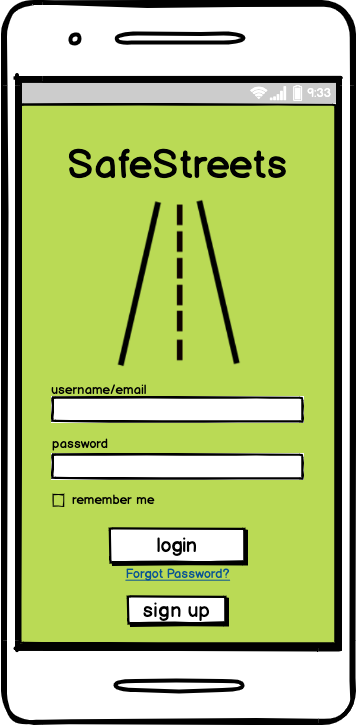
\includegraphics[width=0.7\textwidth]{/mockups/user/loginApp.png}
			\caption{Login Mobile App}
		\end{minipage}\hfill
		\begin{minipage}{0.5\textwidth}
			\centering
			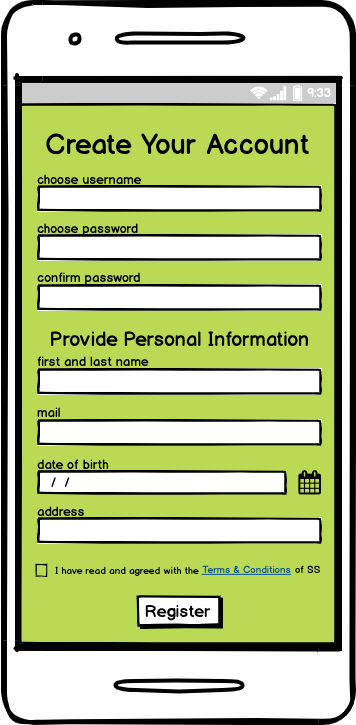
\includegraphics[width=0.7\textwidth]{/mockups/user/registrationApp.png}
			\caption{Registration Mobile App}
		\end{minipage}
	\end{figure}

	\begin{figure}[ht!]
		\centering
		\begin{minipage}{0.5\textwidth}
			\centering
			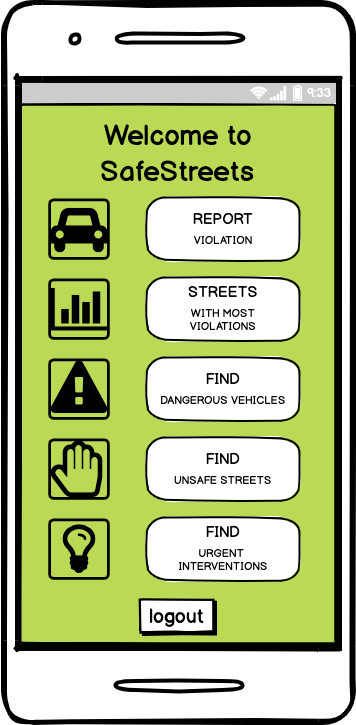
\includegraphics[width=0.7\textwidth]{/mockups/user/homeApp.png}
			\caption{Home Page Mobile App}
		\end{minipage}\hfill
		\begin{minipage}{0.5\textwidth}
			\centering
			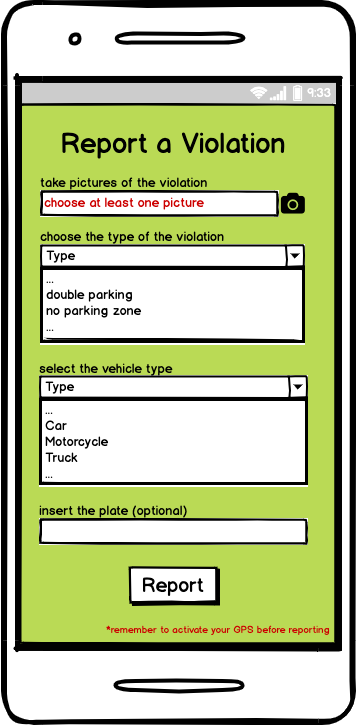
\includegraphics[width=0.7\textwidth]{/mockups/user/notificationApp.png}
			\caption{Notification Mobile App}
		\end{minipage}
	\end{figure}

	\begin{figure}[h!]
		\centering
		\begin{minipage}{0.45\textwidth}
			\centering
			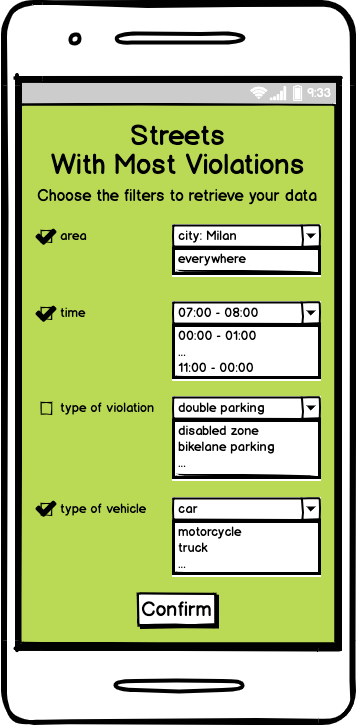
\includegraphics[width=0.7\textwidth]{/mockups/user/violationsFrequencyApp.png}
			\caption{Violations Frequency Mobile App}
		\end{minipage}\hfill
		\begin{minipage}{0.45\textwidth}
			\centering
			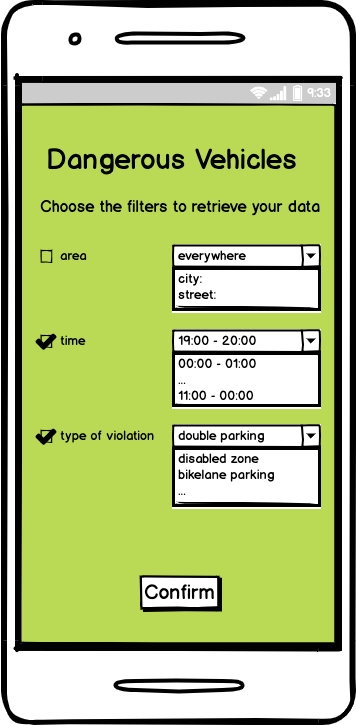
\includegraphics[width=0.7\textwidth]{/mockups/user/dangerousVehiclesApp.png}
			\caption{Dangerous Vehicles Mobile App}
		\end{minipage}
	\end{figure}

	\begin{figure}[h!]
		\centering
		\begin{minipage}{0.45\textwidth}
			\centering
			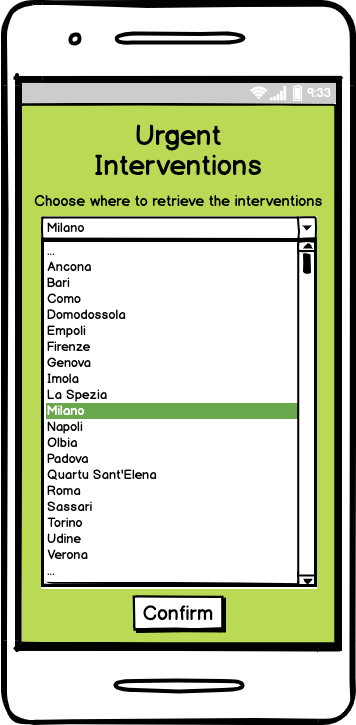
\includegraphics[width=0.7\textwidth]{/mockups/user/urgentInterventionsApp.png}
			\caption{Urgent Interventions Mobile App}
		\end{minipage}\hfill
		\begin{minipage}{0.45\textwidth}
			\centering
			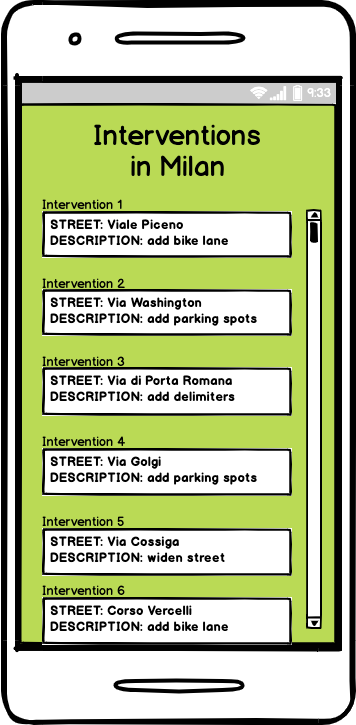
\includegraphics[width=0.7\textwidth]{/mockups/user/interventionsFoundApp.png}
			\caption{Interventions Found Mobile App}
		\end{minipage}
	\end{figure}

	\begin{figure}[h!]
		\centering
		\begin{minipage}{0.45\textwidth}
			\centering
			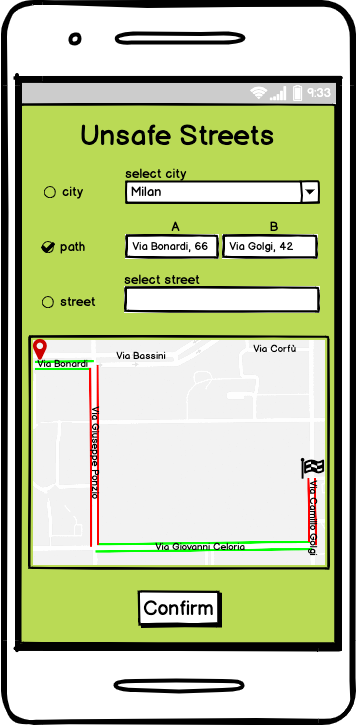
\includegraphics[width=0.7\textwidth]{/mockups/user/unsafeStreetsApp.png}
			\caption{Unsafe Streets Mobile App}
		\end{minipage}
	\end{figure}
	
	\begin{figure}[h!]
		\centering
		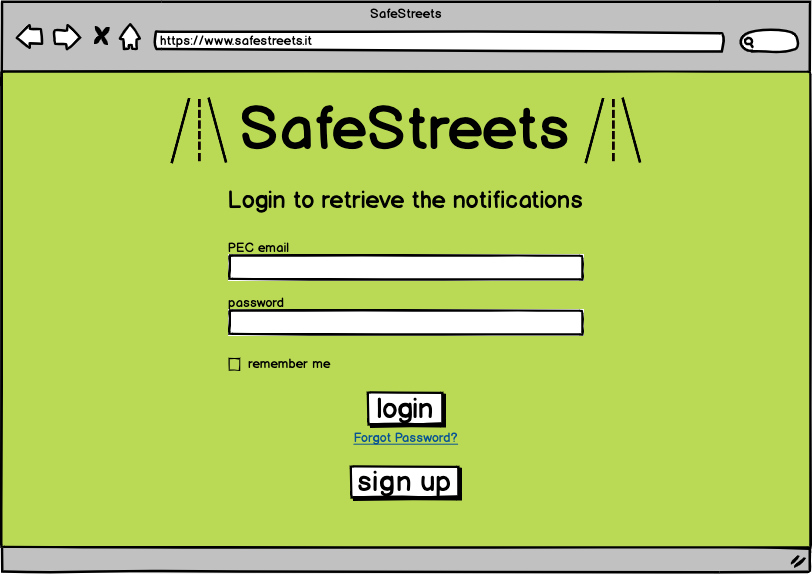
\includegraphics[scale=0.4]{/mockups/authority/loginWeb.png}
		\caption{Login Web App}
	\end{figure}

	\begin{figure}[h!]
		\centering
		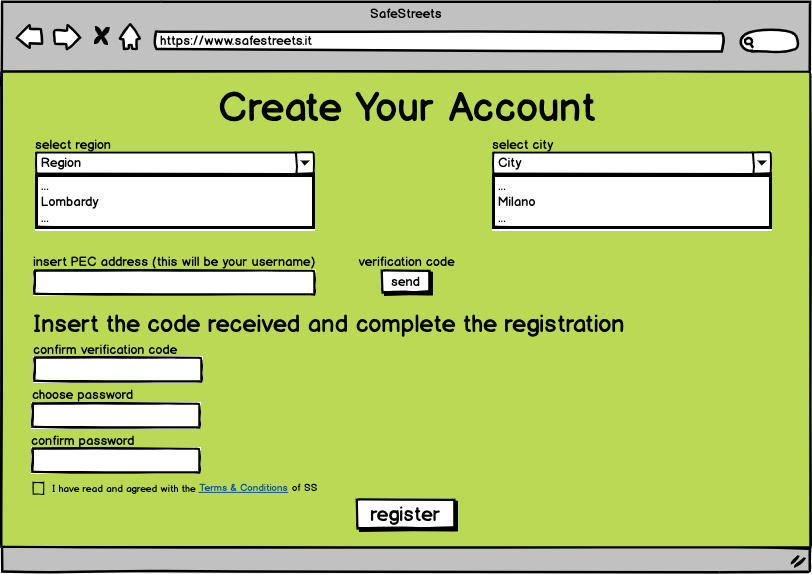
\includegraphics[scale=0.4]{/mockups/authority/registrationWeb.png}
		\caption{Registration Web App}
	\end{figure}

	\begin{figure}[h!]
		\centering
		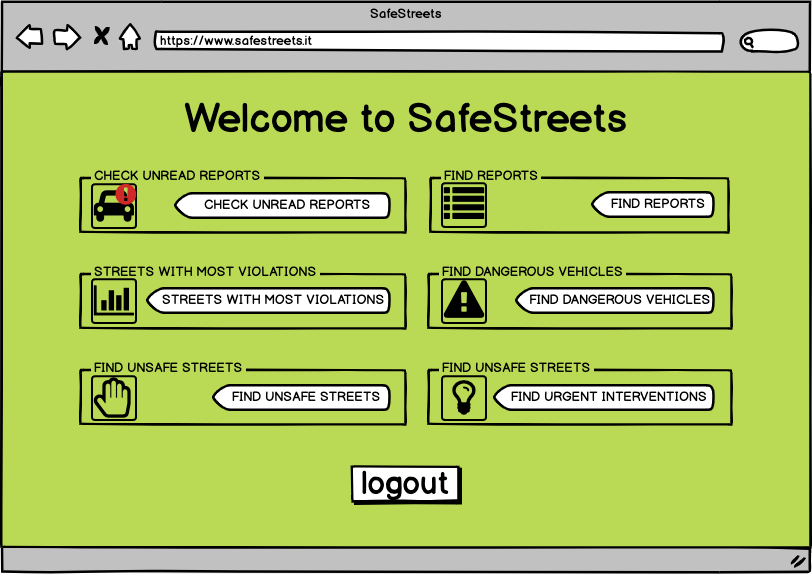
\includegraphics[scale=0.4]{/mockups/authority/homeWeb.png}
		\caption{Home Page Web App}
	\end{figure}
 
 	\begin{figure}[h!]
 		\centering
 		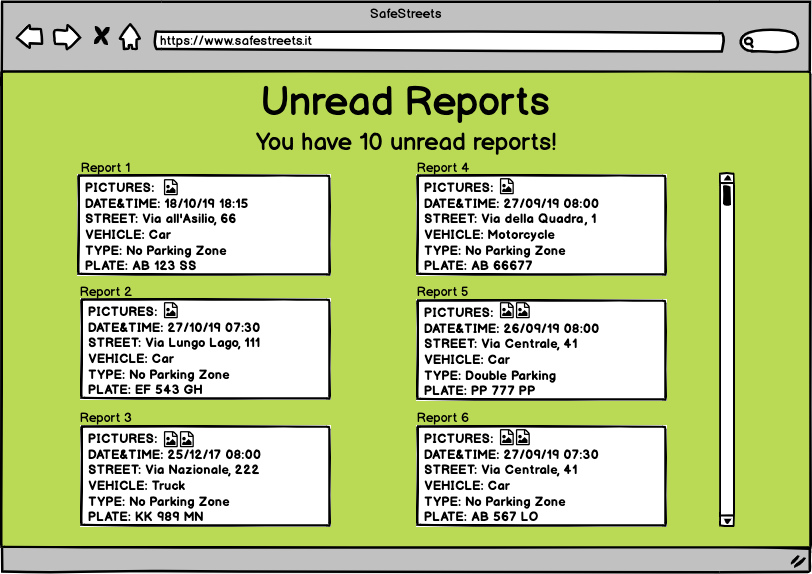
\includegraphics[scale=0.4]{/mockups/authority/unreadReportsWeb.png}
 		\caption{Unread Reports Web App}
 	\end{figure}
 
 	\begin{figure}[h!]
 		\centering
 		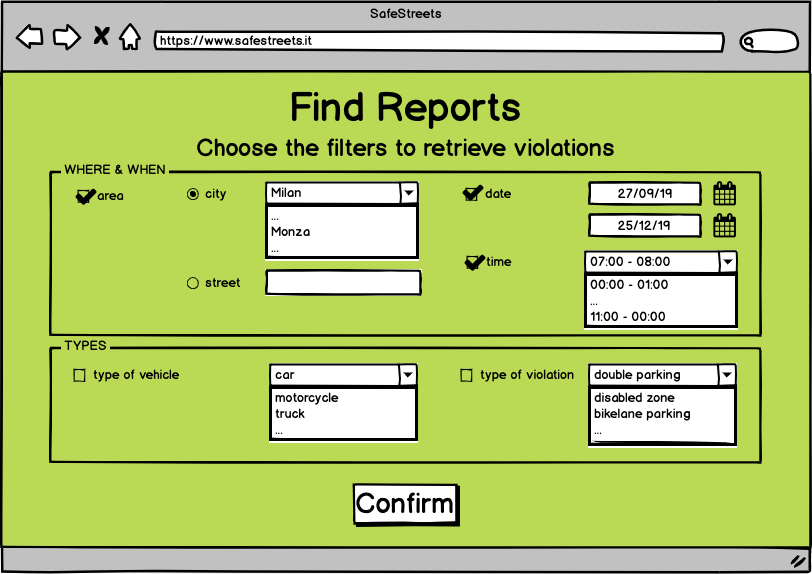
\includegraphics[scale=0.4]{/mockups/authority/findReportsWeb.png}
 		\caption{Find Reports Web App}
 	\end{figure}
 
 	\begin{figure}[h!]
 		\centering
 		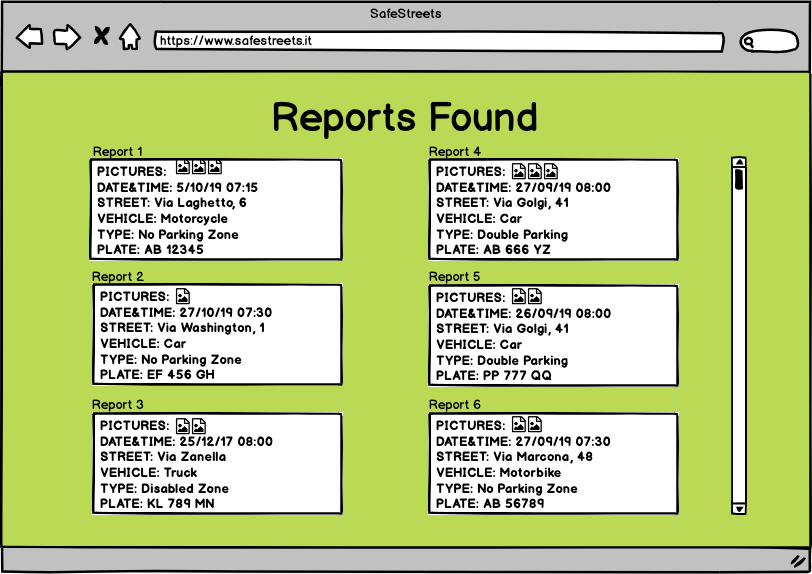
\includegraphics[scale=0.4]{/mockups/authority/reportsFoundWeb.png}
 		\caption{Reports Found Web App}
 	\end{figure}
 
 	\begin{figure}[h!]
 		\centering
 		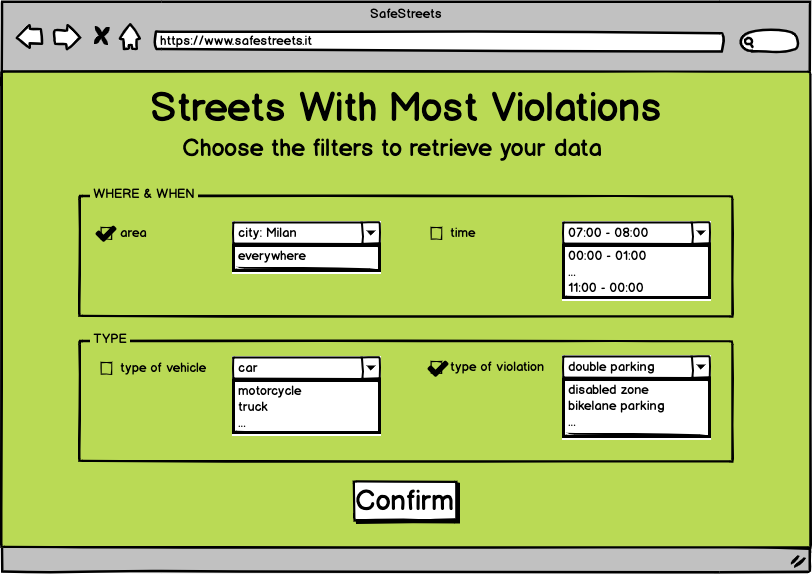
\includegraphics[scale=0.4]{/mockups/authority/violationsFrequencyWeb.png}
 		\caption{Violations Frequency Web App}
 	\end{figure}
 
 	\begin{figure}[h!]
 		\centering
 		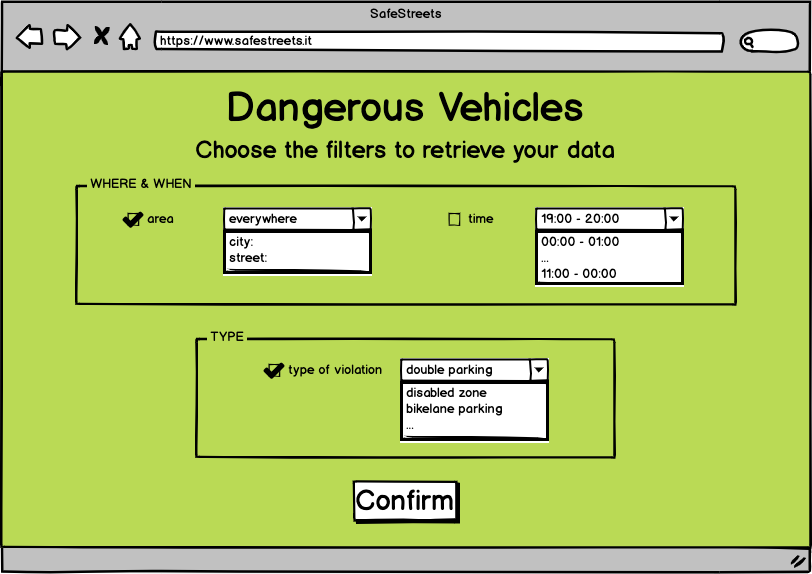
\includegraphics[scale=0.4]{/mockups/authority/dangerousVehiclesWeb.png}
 		\caption{Dangerous Vehicles Web App}
 	\end{figure}
 
 	\begin{figure}[h!]
 		\centering
 		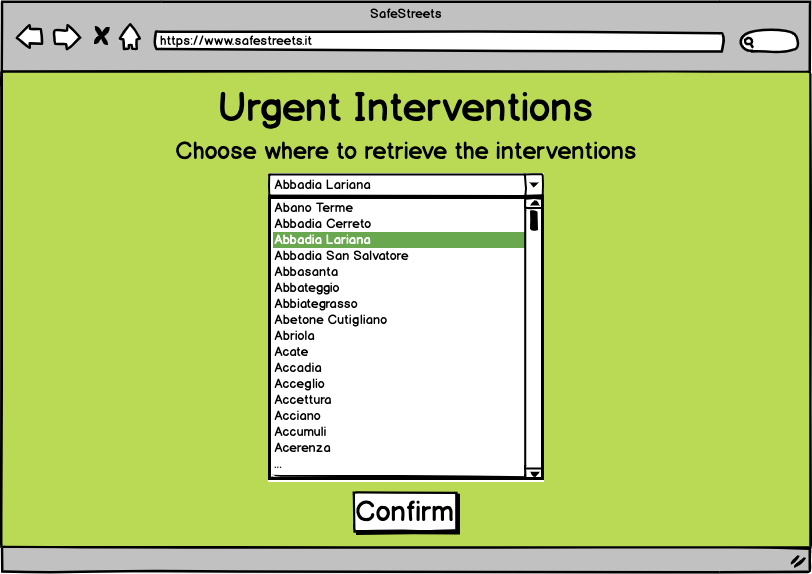
\includegraphics[scale=0.4]{/mockups/authority/urgentInterventionsWeb.png}
 		\caption{Urgent Interventions Web App}
 	\end{figure}
 
	\begin{figure}[h!]
		\centering
		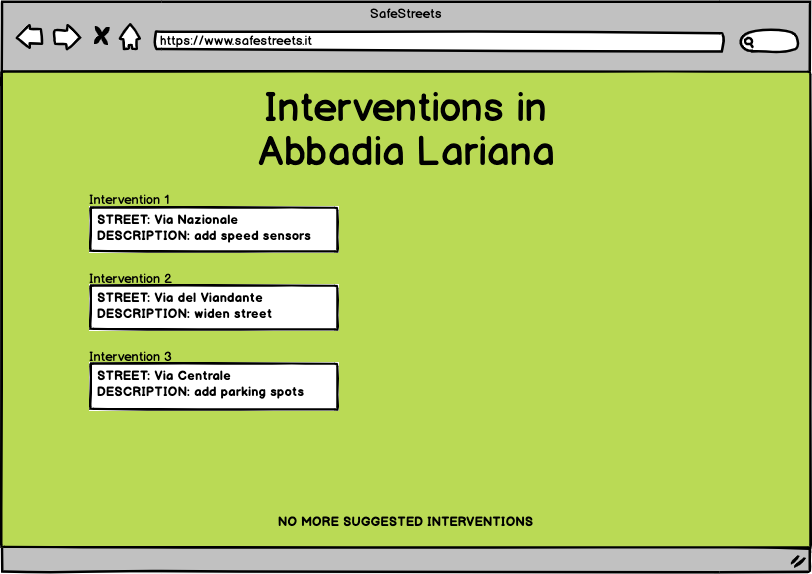
\includegraphics[scale=0.4]{/mockups/authority/interventionsFoundWeb.png}
		\caption{Interventions Found Web App}
	\end{figure} 

	\FloatBarrier

	\begin{figure}[ht!]
		\centering
		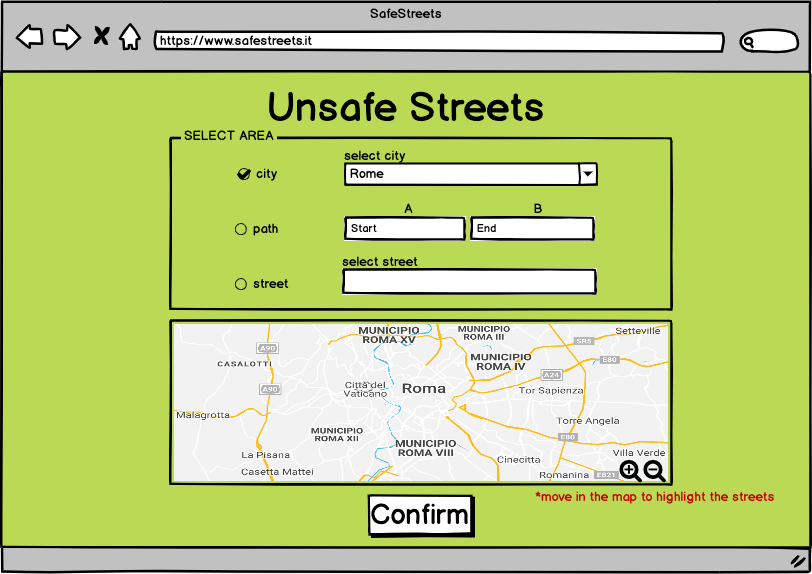
\includegraphics[scale=0.4]{/mockups/authority/unsafeStreetsWeb.png}
		\caption{Unsafe Streets Web App}
	\end{figure}
	
	\subsubsection[Hardware Interfaces]{\hyperlink{toc}{Hardware Interfaces}}
		Hardware interfaces have to be considered on the clients' software in order to interact with the camera and the GPS modules. As described in the section \blueRef{sec:notificationFunction} in fact, a user must always take at least one picture and enable the GPS in order to report a violation. 
		
	\subsubsection[Software Interfaces]{\hyperlink{toc}{Software Interfaces}}
		The interfaces used by SafeStreets to benefit of services provided by external systems are precisely described in the section \blueRef{sec:systemInterfaces}. Internal interfaces instead are needed in particular to manage the DBMS of the system; as described in the section \blueRef{sec:standardCompliance} we will need to manage all the information with different logical models in order to store the different kind of data that the application has to deal with. SafeStreets does not provide APIs to external possible clients.
		
	\subsubsection[Communication Interfaces]{\hyperlink{toc}{Communication Interfaces}}
		An important communication interface that must be considered while developing the system is the one that makes SafeStreets receive the accidents data provided by the municipality. As we described in the global external interface of the authorities we expect to have a system where all of them can publish their accidents as our system will be able to retrieve them.
		
	\newpage

\subsection[Functional Requirements]{\hyperlink{toc}{Functional Requirements}}
	\label{sec:functionalRequirements}
	This subsection aims to give a \emph{complete} description of the \emph{functional requirements} of our system by defining them together with the domain assumptions that satisfy the identified \textbf{goals}.
	
	\subsubsection[Requirements]{\hyperlink{toc}{Requirements}}
		\begin{enumerate}[label=\textbf{R\arabic*}]
			\item \label{req:userReg} The system must allow users to register.
			\item \label{req:authorityReg} The system must allow authorities to register.
			\item \label{req:userLogin} The system must allow the user to log in.
			\item \label{req:authorityLogin} The system must allow authorities to log in.
			\item \label{req:uniqueName} The system must guarantee that each username is unique.
			\item \label{req:saveRegData} The system must save the customers registration data.
			\item \label{req:specialCharacters} The system must prevent users to use special characters in their username.
			\item \label{req:takePictures} The system must allow users to take pictures of the violation they want to report.
			\item \label{req:dateTime} The system must retrieve date and time while the user reports a violation.
			\item \label{req:gpsPosition} The system must retrieve the GPS position while the user reports a violation.
			\item \label{req:violationType} The system must allow users to insert the type of violation they’re reporting.
			\item \label{req:vehicleType} The system must allow users to insert the type of the vehicles they’re reporting.
			\item \label{req:plateNumber} The system must allow users to insert the license plate number of the vehicle they are reporting.
			\item \label{req:readPlate} The system must read the license plate from every picture sent by the user.
			\item \label{req:storeViolation} The system must store the data received along with the name of the street where the violation occurred.
			\item \label{req:streetName} The system must be able to retrieve the name of the street from the GPS coordinates.
			\item \label{req:notifyAuthority} The system must be able to show authorities all the violation reports sent by users.
			\item \label{req:mineData} The system must be able to mine the stored violation reports.
			\item \label{req:cityFilter} The system must allow the customer to filter by city.
			\item \label{req:streetFilter} The system must allow the customer to filter by street.
			\item \label{req:pathFilter} The system must allow the customer to filter by path.
			\item \label{req:violationFilter} The system must allow the customer to filter by type of violation.
			\item \label{req:timeFilter} The system must allow the customer to filter by time slot.
			\item \label{req:dateFilter} The system must allow the authority to filter by date intervals.
			\item \label{req:vehicleFilter} The system must allow the customer to filter by type of vehicle.
			\item \label{req:sortedResult} The system must be able to sort streets by number of violations.
			\item \label{req:sortedVehicles} The system must be able to sort types of vehicle by number of violations they make.
			\item \label{req:visibility} The system must be able to provide different levels of visibility.
			\item \label{req:accidentsData} The system must be able to store and manage data about accidents, if provided by the authority.
			\item \label{req:crossData} The system must be able to cross accidents data with violations one.
			\item \label{req:safeStreet} The system must be able to determine whether a street is safe or not.
			\item \label{req:cityStreets} The system must be able to access all the available maps.
			\item \label{req:pathFinder} The system must find a path between two given points in a map.
			\item \label{req:colorMap} The system must be able to color the streets in a map according to their safety.
			\item \label{req:interventions} The system must be able to determine the most urgent interventions in a street.	
		\end{enumerate}
	
	\subsubsection[Goals]{\hyperlink{toc}{Goals}}
		\label{sec:goalSatisfaction}
		\begin{description}
			\setlength\itemsep{0.7cm}
			\item \blueRef{goal:notification}\ \textbf{Users should be able to notify authorities when traffic violations occur, in particular parking violations.}
				\begin{description}
					\item \blueRef{req:userReg}\ The system must allow users to register.
					\item \blueRef{req:authorityReg}\ The system must allow authorities to register.
					\item \blueRef{req:userLogin}\ The system must allow the user to log in.
					\item \blueRef{req:authorityLogin}\ The system must allow authorities to log in.
					\item \blueRef{req:uniqueName}\ The system must guarantee that each username is unique.
					\item \blueRef{req:saveRegData}\ The system must save the customers' registration data.
					\item \blueRef{req:specialCharacters}\ The system must prevent users to use special characters in their username.
					\item \blueRef{req:takePictures}\ The system must allow users to take pictures of the violation they want to report.
					\item \blueRef{req:dateTime}\ The system must retrieve date and time while the user reports a violation.
					\item \blueRef{req:gpsPosition}\ The system must retrieve the GPS position while the user reports a violation.
					\item \blueRef{req:violationType}\ The system must allow users to insert the type of violation they’re reporting.
					\item \blueRef{req:vehicleType}\ The system must allow users to insert the type of the vehicles they’re reporting.
					\item \blueRef{req:plateNumber}\ The system must allow users to insert the license plate number of the vehicle they are reporting.
					\item \blueRef{req:readPlate}\ The system must read the license plate from every picture sent by the user.
					\item \blueRef{req:storeViolation}\ The system must store the data received along with the name of the street where the violation occurred.
					\item \blueRef{req:streetName}\ The system must be able to retrieve the name of the street from the GPS coordinates.
					\item \blueRef{req:notifyAuthority}\ The system must be able to show authorities all the violation reports sent by users.
					\item \blueRef{dom:correctRegistration}\ Customers always insert correct data while registering to SafeStreets.
					\item \blueRef{dom:correctViolation}\ Users always insert correct data while reporting violations to SafeStreets.
					\item \blueRef{dom:pecKnown}\ The association between cities and PEC is well-known by SafeStreets.
					\item \blueRef{dom:uniquePec}\ PEC addresses are unique.
					\item \blueRef{dom:specialCharacters}\ Special characters are all the characters that are not letters nor numbers.
					\item \blueRef{dom:correctDateTime}\ Date and time on the devices on which SafeStreets runs are always correct.
					\item \blueRef{dom:gpsAccuracy}\ The GPS module of the devices on which SafeStreets runs always works correctly and has an accuracy of 2 meters.
					\item \blueRef{dom:correctCamera}\ The camera module of the devices on which SafeStreets runs always works correctly.
					\item \blueRef{dom:correctInternet}\ Internet connection works always without errors.
					\item \blueRef{dom:italy}\ The system is assumed to work in Italy.
					\item \blueRef{dom:italyMaps}\ Maps of Italy are well known, complete and up to date.
					\item \blueRef{dom:nonameStreets}\ There are no streets without a name.
					\item \blueRef{dom:noMaliciousPlates}\ No one physically and maliciously replaces license plates.
					\item \blueRef{dom:nosameStreets}\ In a city there are not streets with the same name.
					\item \blueRef{dom:streetCity}\ Every street belongs exactly to one city.
					\item \blueRef{dom:nomultipleViolations}\ No multiple violations of the same vehicle occur in the same place at the same time.
				\end{description}
					
			\item \blueRef{goal:mining}\ \textbf{Users and authorities should be able to mine the information stored by SafeStreets, with different levels of visibility.}
				\begin{description}
					\setlength\itemsep{0.7cm}
					\item \blueRef{goal:miningA}\ \textbf{Users and authorities should be able to know where the highest number of violations occur.}
						\begin{description}
							\item \blueRef{req:userReg}\ The system must allow users to register.
							\item \blueRef{req:authorityReg}\ The system must allow authorities to register.
							\item \blueRef{req:userLogin}\ The system must allow the user to log in.
							\item \blueRef{req:authorityLogin}\ The system must allow authorities to log in.
							\item \blueRef{req:saveRegData}\ The system must save the customers registration data.
							\item \blueRef{req:storeViolation}\ The system must store the data received along with the name of the street where the violation occurred.
							\item \blueRef{req:mineData}\ The system must be able to mine the stored violation reports.
							\item \blueRef{req:cityFilter}\ The system must allow the customer to filter by city.
							\item \blueRef{req:violationFilter}\ The system must allow the customer to filter by type of violation.
							\item \blueRef{req:timeFilter}\ The system must allow the customer to filter by time slot.
							\item \blueRef{req:vehicleFilter}\ The system must allow the customer to filter by type of vehicle.
							\item \blueRef{req:sortedResult}\ The system must be able to sort streets by number of violations.
							\item \blueRef{dom:correctRegistration}\ Customers always insert correct data while registering to SafeStreets.
							\item \blueRef{dom:correctViolation}\ Users always insert correct data while reporting violations to SafeStreets.
							\item \blueRef{dom:pecKnown}\ The association between cities and PEC is well-known by SafeStreets.
							\item \blueRef{dom:uniquePec}\ PEC addresses are unique.
							\item \blueRef{dom:specialCharacters}\ Special characters are all the characters that are not letters nor numbers.
							\item \blueRef{dom:correctInternet}\ Internet connection works always without errors.
							\item \blueRef{dom:italyMaps}\ Maps of Italy are well known, complete and up to date.
							\item \blueRef{dom:nonameStreets}\ There are no streets without a name.
							\item \blueRef{dom:nosameStreets}\ In a city there are not streets with the same name.
							\item \blueRef{dom:streetCity}\ Every street belongs exactly to one city.
						\end{description}
					\item \blueRef{goal:miningB}\ \textbf{Users and authorities should be able to know what types of vehicle make the most violations.}
						\begin{description}
							\item \blueRef{req:userReg}\ The system must allow users to register.
							\item \blueRef{req:authorityReg}\ The system must allow authorities to register.
							\item \blueRef{req:userLogin}\ The system must allow the user to log in.
							\item \blueRef{req:authorityLogin}\ The system must allow authorities to log in.
							\item \blueRef{req:saveRegData}\ The system must save the customers registration data.
							\item \blueRef{req:storeViolation}\ The system must store the data received along with the name of the street where the violation occurred.
							\item \blueRef{req:mineData}\ The system must be able to mine the stored violation reports.
							\item \blueRef{req:cityFilter}\ The system must allow the customer to filter by city.
							\item \blueRef{req:violationFilter}\ The system must allow the customer to filter by type of violation.
							\item \blueRef{req:sortedVehicles}\ The system must be able to sort types of vehicle by number of violations they make.
							\item \blueRef{dom:correctRegistration}\ Customers always insert correct data while registering to SafeStreets.
							\item \blueRef{dom:correctViolation}\ Users always insert correct data while reporting violations to SafeStreets.
							\item \blueRef{dom:pecKnown}\ The association between cities and PEC is well-known by SafeStreets.
							\item \blueRef{dom:uniquePec}\ PEC addresses are unique.
							\item \blueRef{dom:specialCharacters}\ Special characters are all the characters that are not letters nor numbers.
							\item \blueRef{dom:correctInternet}\ Internet connection works always without errors.
							\item \blueRef{dom:italyMaps}\ Maps of Italy are well known, complete and up to date.
							\item \blueRef{dom:nonameStreets}\ There are no streets without a name.
							\item \blueRef{dom:nosameStreets}\ In a city there are not streets with the same name.
							\item \blueRef{dom:streetCity}\ Every street belongs exactly to one city.
						\end{description}
					\item \blueRef{goal:miningC}\ \textbf{Authorities should be able to consult every violation report sent by users.}
						\begin{description}
							\item \blueRef{req:authorityReg}\ The system must allow authorities to register.
							\item \blueRef{req:authorityLogin}\ The system must allow authorities to log in.
							\item \blueRef{req:saveRegData}\ The system must save the customers registration data.
							\item \blueRef{req:storeViolation}\ The system must store the data received along with the name of the street where the violation occurred.
							\item \blueRef{req:mineData}\ The system must be able to mine the stored violation reports.
							\item \blueRef{req:cityFilter}\ The system must allow the customer to filter by city.
							\item \blueRef{req:streetFilter}\ The system must allow the customer to filter by street.
							\item \blueRef{req:violationFilter}\ The system must allow the customer to filter by type of violation.
							\item \blueRef{req:timeFilter}\ The system must allow the customer to filter by time slot.
							\item \blueRef{req:dateFilter}\ The system must allow the authority to filter by date intervals.
							\item \blueRef{req:vehicleFilter}\ The system must allow the customer to filter by type of vehicle.
							\item \blueRef{req:visibility}\ The system must be able to provide different levels of visibility.
							\item \blueRef{dom:correctRegistration}\ Customers always insert correct data while registering to SafeStreets.
							\item \blueRef{dom:correctViolation}\ Users always insert correct data while reporting violations to SafeStreets.
							\item \blueRef{dom:pecKnown}\ The association between cities and PEC is well-known by SafeStreets.
							\item \blueRef{dom:uniquePec}\ PEC addresses are unique.
							\item \blueRef{dom:specialCharacters}\ Special characters are all the characters that are not letters nor numbers.
							\item \blueRef{dom:correctInternet}\ Internet connection works always without errors.
							\item \blueRef{dom:italyMaps}\ Maps of Italy are well known, complete and up to date.
							\item \blueRef{dom:nonameStreets}\ There are no streets without a name.
							\item \blueRef{dom:nosameStreets}\ In a city there are not streets with the same name.
							\item \blueRef{dom:streetCity}\ Every street belongs exactly to one city.
						\end{description}
				\end{description}
			\item \blueRef{goal:safety}\ \textbf{Users and authorities should be able to know which streets are safe and which ones are not.} 
				\begin{description}
					\item \blueRef{req:userReg}\ The system must allow users to register.
					\item \blueRef{req:authorityReg}\ The system must allow authorities to register.
					\item \blueRef{req:userLogin}\ The system must allow the user to log in.
					\item \blueRef{req:authorityLogin}\ The system must allow authorities to log in.
					\item \blueRef{req:saveRegData}\ The system must save the customers registration data.
					\item \blueRef{req:storeViolation}\ The system must store the data received along with the name of the street where the violation occurred.
					\item \blueRef{req:crossData}\ The system must be able to cross accidents data with violations one.
					\item \blueRef{req:safeStreet}\ The system must be able to determine whether a street is safe or not.
					\item \blueRef{req:accidentsData}\ The system must be able to store and manage data about accidents, if provided by the authority.
					\item \blueRef{req:cityStreets} The system must be able to access all the available maps.
					\item \blueRef{req:pathFinder} The system must find a path between two given points in a map.
					\item \blueRef{req:colorMap} The system must be able to color the streets in a map according to their safety.
					\item \blueRef{req:cityFilter} The system must allow the customer to filter by city.
					\item \blueRef{req:streetFilter} The system must allow the customer to filter by street.
					\item \blueRef{req:pathFilter} The system must allow the customer to filter by path.
					\item \blueRef{dom:correctRegistration}\ Customers always insert correct data while registering to SafeStreets.
					\item \blueRef{dom:correctViolation}\ Users always insert correct data while reporting violations to SafeStreets.
					\item \blueRef{dom:pecKnown}\ The association between cities and PEC is well-known by SafeStreets.
					\item \blueRef{dom:uniquePec}\ PEC addresses are unique.
					\item \blueRef{dom:specialCharacters}\ Special characters are all the characters that are not letters nor numbers.
					\item \blueRef{dom:correctInternet}\ Internet connection works always without errors.
					\item \blueRef{dom:italyMaps}\ Maps of Italy are well known, complete and up to date.
					\item \blueRef{dom:nonameStreets}\ There are no streets without a name.
					\item \blueRef{dom:nosameStreets}\ In a city there are not streets with the same name.
					\item \blueRef{dom:streetCity}\ Every street belongs exactly to one city.
					\item \blueRef{dom:correctAccidents}\ Accidents data provided by municipalities are always correct.
				\end{description}	
			\item \blueRef{goal:intervention}\ \textbf{Users and authorities should be able to know the possible interventions that could be done in a city.}
				\begin{description}
					\item \blueRef{req:userReg}\ The system must allow users to register.
					\item \blueRef{req:authorityReg}\ The system must allow authorities to register.
					\item \blueRef{req:userLogin}\ The system must allow the user to log in.
					\item \blueRef{req:authorityLogin}\ The system must allow authorities to log in.
					\item \blueRef{req:saveRegData}\ The system must save the customers registration data.
					\item \blueRef{req:storeViolation}\ The system must store the data received along with the name of the street where the violation occurred.
					\item \blueRef{req:crossData}\ The system must be able to cross accidents data with violations one.
					\item \blueRef{req:accidentsData}\ The system must be able to store and manage data about accidents, if provided by the authority.
					\item \blueRef{req:cityStreets} The system must be able to access all the available maps.
					\item \blueRef{req:interventions} The system must be able to determine the most urgent interventions in a street.
					\item \blueRef{req:cityFilter} The system must allow the customer to filter by city.
					\item \blueRef{dom:correctRegistration}\ Customers always insert correct data while registering to SafeStreets.
					\item \blueRef{dom:correctViolation}\ Users always insert correct data while reporting violations to SafeStreets.
					\item \blueRef{dom:pecKnown}\ The association between cities and PEC is well-known by SafeStreets.
					\item \blueRef{dom:uniquePec}\ PEC addresses are unique.
					\item \blueRef{dom:specialCharacters}\ Special characters are all the characters that are not letters nor numbers.
					\item \blueRef{dom:correctInternet}\ Internet connection works always without errors.
					\item \blueRef{dom:italyMaps}\ Maps of Italy are well known, complete and up to date.
					\item \blueRef{dom:nonameStreets}\ There are no streets without a name.
					\item \blueRef{dom:nosameStreets}\ In a city there are not streets with the same name.
					\item \blueRef{dom:streetCity}\ Every street belongs exactly to one city.
					\item \blueRef{dom:correctAccidents}\ Accidents data provided by municipalities are always correct.	
				\end{description}		
		\end{description}
	
		\newpage

\subsection[Use Cases Identification]{\hyperlink{toc}{Use Cases Identification}}
	In the following subsection the usage of the system is going to be described first with a general description using scenarios and then in a more specific way using use case diagrams. These diagrams are going to be described only once for the functionalities that totally coincide between users and authorities. Hence only the ones where critical behaviors are needed to be considered are duplicated highlighting these parts. The subsection ends with the traceability matrix that allows to define the correspondence between \emph{requirements, use cases and scenarios.}
	
	\subsubsection[Scenarios]{\hyperlink{toc}{Scenarios}}
		Consider these scenarios in order to clarify the usage of the system and the further description with use case diagrams.
		
		\paragraph{User}
		\begin{enumerate}[label=\textbf{US\arabic*}]
			\item \label{sce:notification} A man living in Milan has a son with disabilities named Gianluca. His son in particular suffers leg paralysis and therefore is confined to a wheelchair. Since he wants his son to live his life at its fullest, he made him take up para table tennis, the variant of table tennis designed for people with disabilities. The problem is, although few places are reserved for people with disabilities, there’s no much parking in the area where training sessions are held, and so, unfortunately, people get to park in reserved spots anyway, even if they’re not allowed to. Gianluca’s father got really annoyed because of this situation, especially because sidewalks are not in good conditions and therefore he can’t park too far away. In addition, policemen never show up in the area. He discovers SafeStreets, and starts reporting to the authorities all of those vehicles that have not exposed the pass for people with disabilities, by sending pictures of those vehicles. He makes sure that the license plate is readable and hopes that local police will take action.
			
			\item \label{sce:basicUser} A group of guys fond of bicycles and competitions is going to organize a treasure hunt in Citta Studi. In this kind of game the competitors have to seek the treasures and who first finds all of them wins. The organizers must position the treasures in each area where the less number of parking violations occur to avoid bikers getting hurt when reaching them on a very high speed. Typically each organizer has an area in which he has to decide where to put the treasure. Using SafeStreet’s basic functionality each of them can select Milan as the filter for the area together with the time lapse in which they expect the bikers to arrive and determine the best street in their area where the less number of violations occur.
			
			\item \label{sce:advancedUser} A sportive family from Milan decides to go by bike on a weekend trip to the Idroscalo. Knowing that the bicycle lane from Milan to Idroscalo gets interrupted once reached the city of Novegro, they have to decide which street is better to reach Idroscalo safely. Thanks to SafeStreets advanced functionality they can select the path and choose whether to continue taking a short part aside the highway or to get inside Novegro and enter the park from the bottom. 
		\end{enumerate}
	
		\paragraph{Authority}
		\begin{enumerate}[label=\textbf{AS\arabic*}]
			\item \label{sce:findReports} Circolo Vela Bellano (CVB) is a sailing club located on the high part of the Como lake. Every year it organizes a competition named \emph{Coppa Bellano} where all members of the club tend to participate. CVB every year tries to ask to the municipality if for the entire week-end when the competition is organized the competitors can be enabled to park also on the spots for the residents (highly more than the free ones definitely not enough for the hundreds of people coming). This year, fortunately, the municipality of Bellano has decided to take action for this request, but first wants to be sure that the problem is really the one reported by the club. To solve this doubt it registers to SafeStreets using the PEC address and thanks to the \emph{Find Reports} functionality it can filter all the violations that occurred the previous year when the competition took place. The high level of details in each violation shows that the plates numbers are all of vehicles owned by people not from Bellano. Hence the municipality decides to accomplish the desire of the club understanding that it is better to encourage the hundreds of people arriving in a small town like Bellano rather than giving them fines!
			
			\item \label{sce:basicAuthority} Cesate Public Library is the only library in Cesate and is usually open for too little time. The problem is the municipality of Cesate has lately become short on money and therefore can’t pay enough people to work in there. Students living in that small town have no other place to study in silence and if they really need it, they can do nothing but go to Arese or Saronno, that have really big libraries but are only reachable after 15 minutes by car. Since Lombardy Region hasn’t got any plan to give funds to Cesate, the municipality, that really cares about the future of its young citizens, decides to go his own way and tries to give the most traffic tickets it can. In order to do this without wasting time, the municipality uses SafeStreets to figure out where the highest number of traffic violations occur, and then sends policemen in those streets to give fines.
			
			\item \label{sce:advancedAuthority} It’s almost election time in Cesate and the outgoing local administration would like to be elected again for their second mandate. In order to gain the highest number of votes in the upcoming elections, the party decides that finally it’s time to make some useful public works. The problem is they really have no clue about what their citizens need most, but fortunately, Ascanio, the City council member to the transports, knows SafeStreets. He is able to get the list of the most urgent works, according to SafeStreets. He in particular finds out that an old street that links the old part of the city to the newest one is the place where a lot of cyclists fall because of potholes. They asphalt that street and are elected again.
		\end{enumerate}
	
		\newpage
		
	\subsubsection[Use Cases Diagrams]{\hyperlink{toc}{Use Case Diagram}}
		The following diagram is a high-level description of the possible interactions of actors with the system and highlights the different use case in which actors are involved.
		
		\vspace{0.3cm}
		
		\begin{figure}[h!]
			\centering
			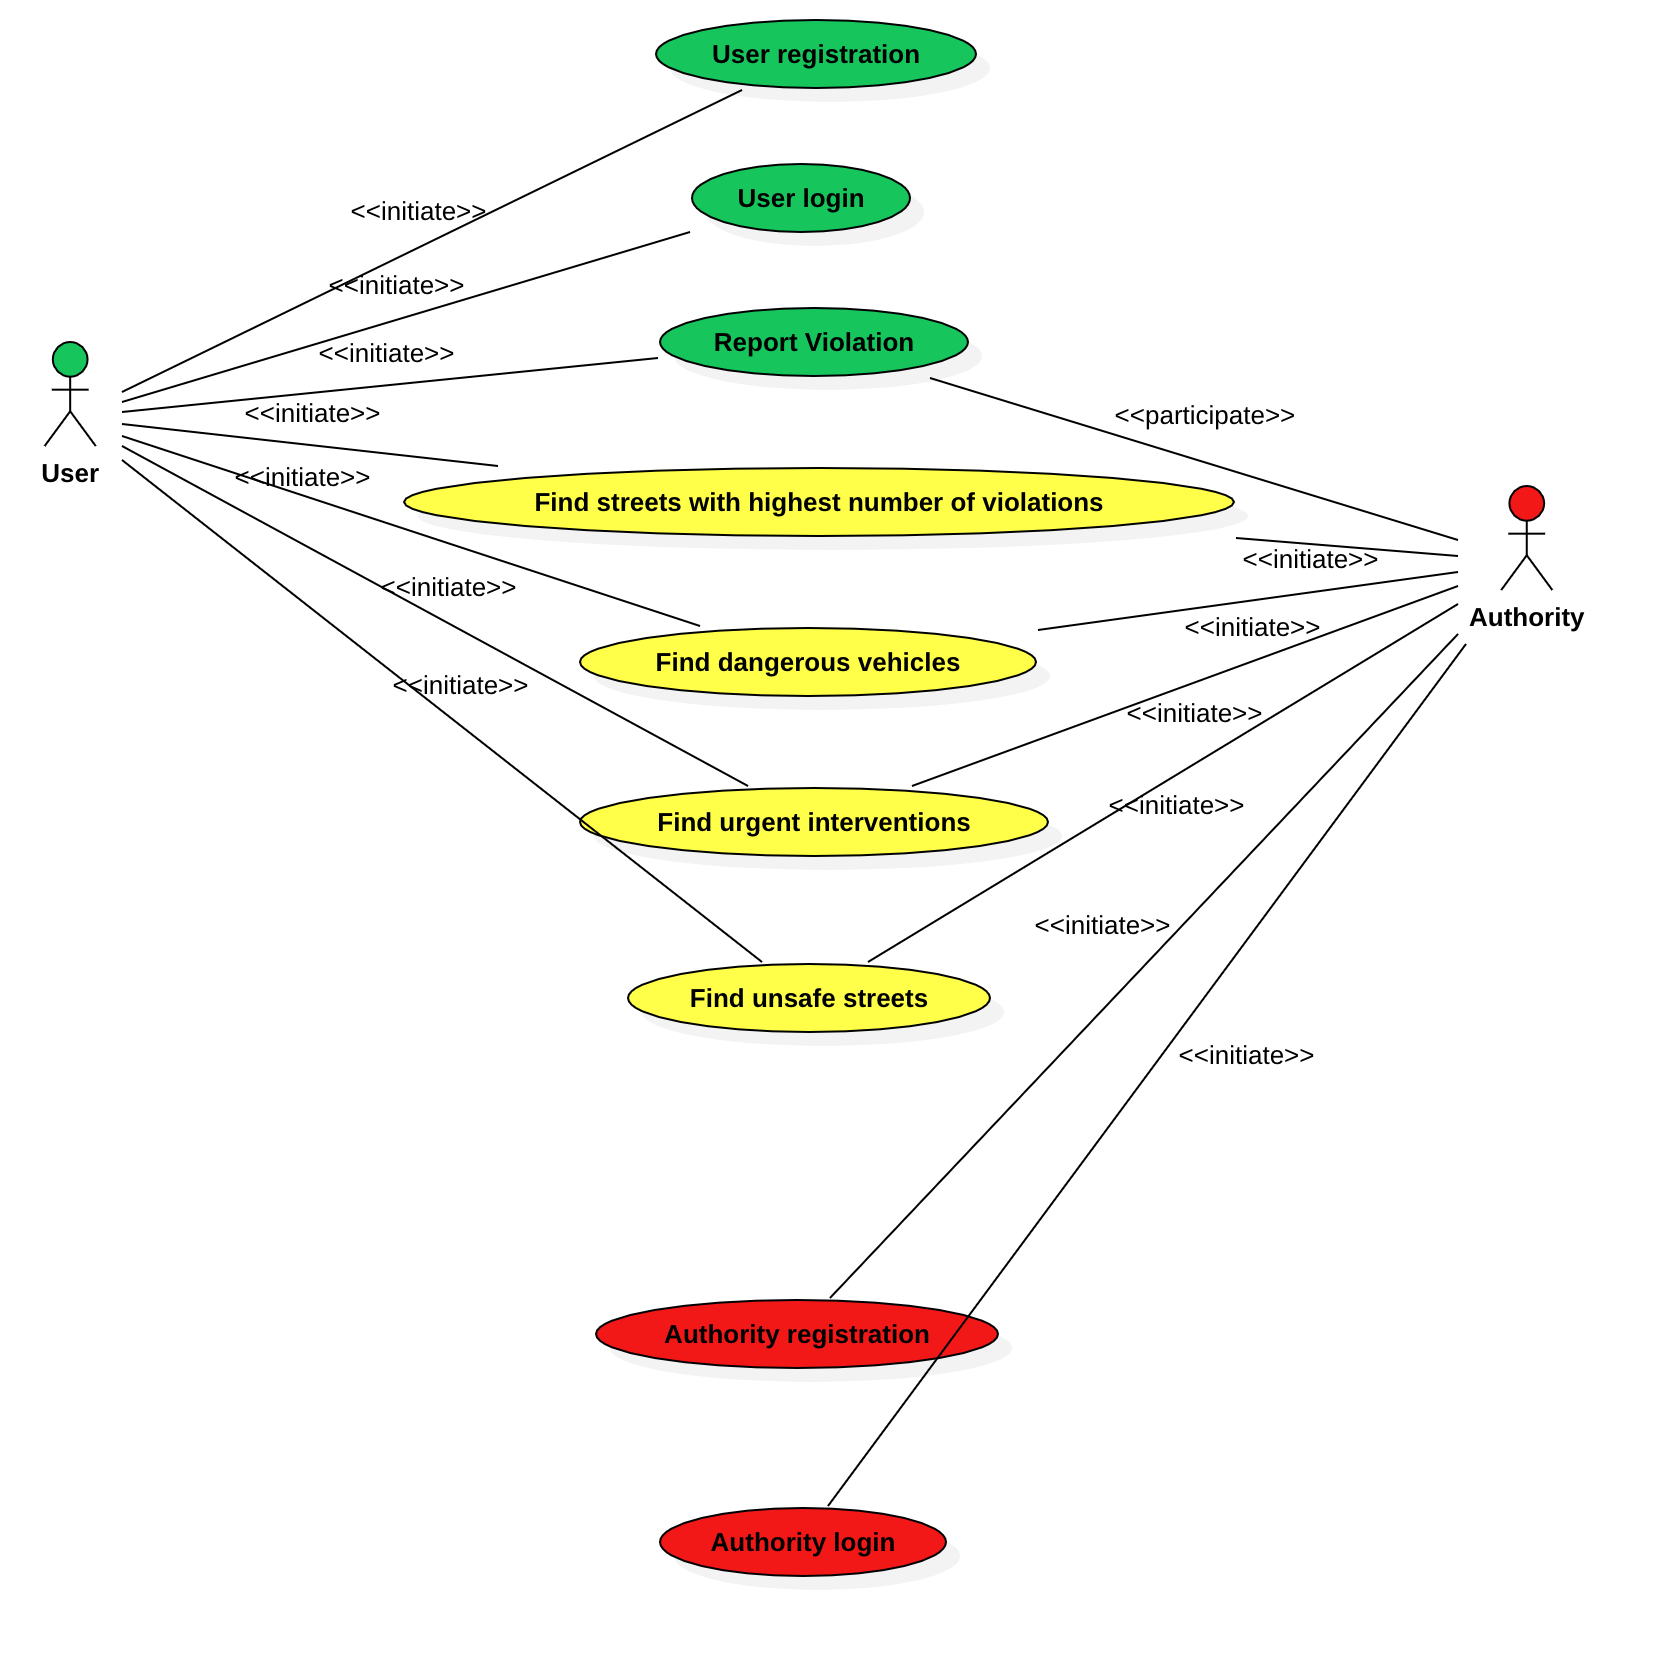
\includegraphics[scale=0.23]{/diagrams/usecaseDiagramModel.png}
			\caption{Use Case Diagram}
		\end{figure}
	
		\FloatBarrier
	
	\subsubsection[Use Cases Description]{\hyperlink{toc}{Use Cases Description}}
		\label{sec:useCases}
		
		\paragraph{User}
		\begin{enumerate}
			\item \textbf{User Registration} 
				\begin{longtable}{p{0.26\linewidth}p{0.75\linewidth}}
					\toprule
					\textbf{Name} & \textbf{User Registration} \\
					\midrule
					\textbf{Actors} & User \\
					\midrule
					\textbf{Entry conditions} & The mobile application has started \\
					\midrule
					\textbf{Flow of events} & 
					\begin{enumerate}
						\item The user chooses the sign up option
						\item The user chooses a username and a password
						\item The user inserts his name, surname and address
						\item The user accepts the \emph{Terms and Conditions} of SafeStreets
						\item The user submits the form
						\item The system checks the username to be unique
						\item The system saves the user data
					\end{enumerate} \\
					\midrule
					\textbf{Exit conditions} & The user is registered in the system\\
					\midrule
					\textbf{Exceptions} & 
					\begin{itemize}
						\item If the username inserted by the user is already used by another user, or if the username contains any special character, the system displays an error message asking the user to insert a different one
					\end{itemize} \\
					\bottomrule
					\caption{\emph{User Registration} use case description}
				\end{longtable}
			
				\begin{figure}[h]
					\centering
					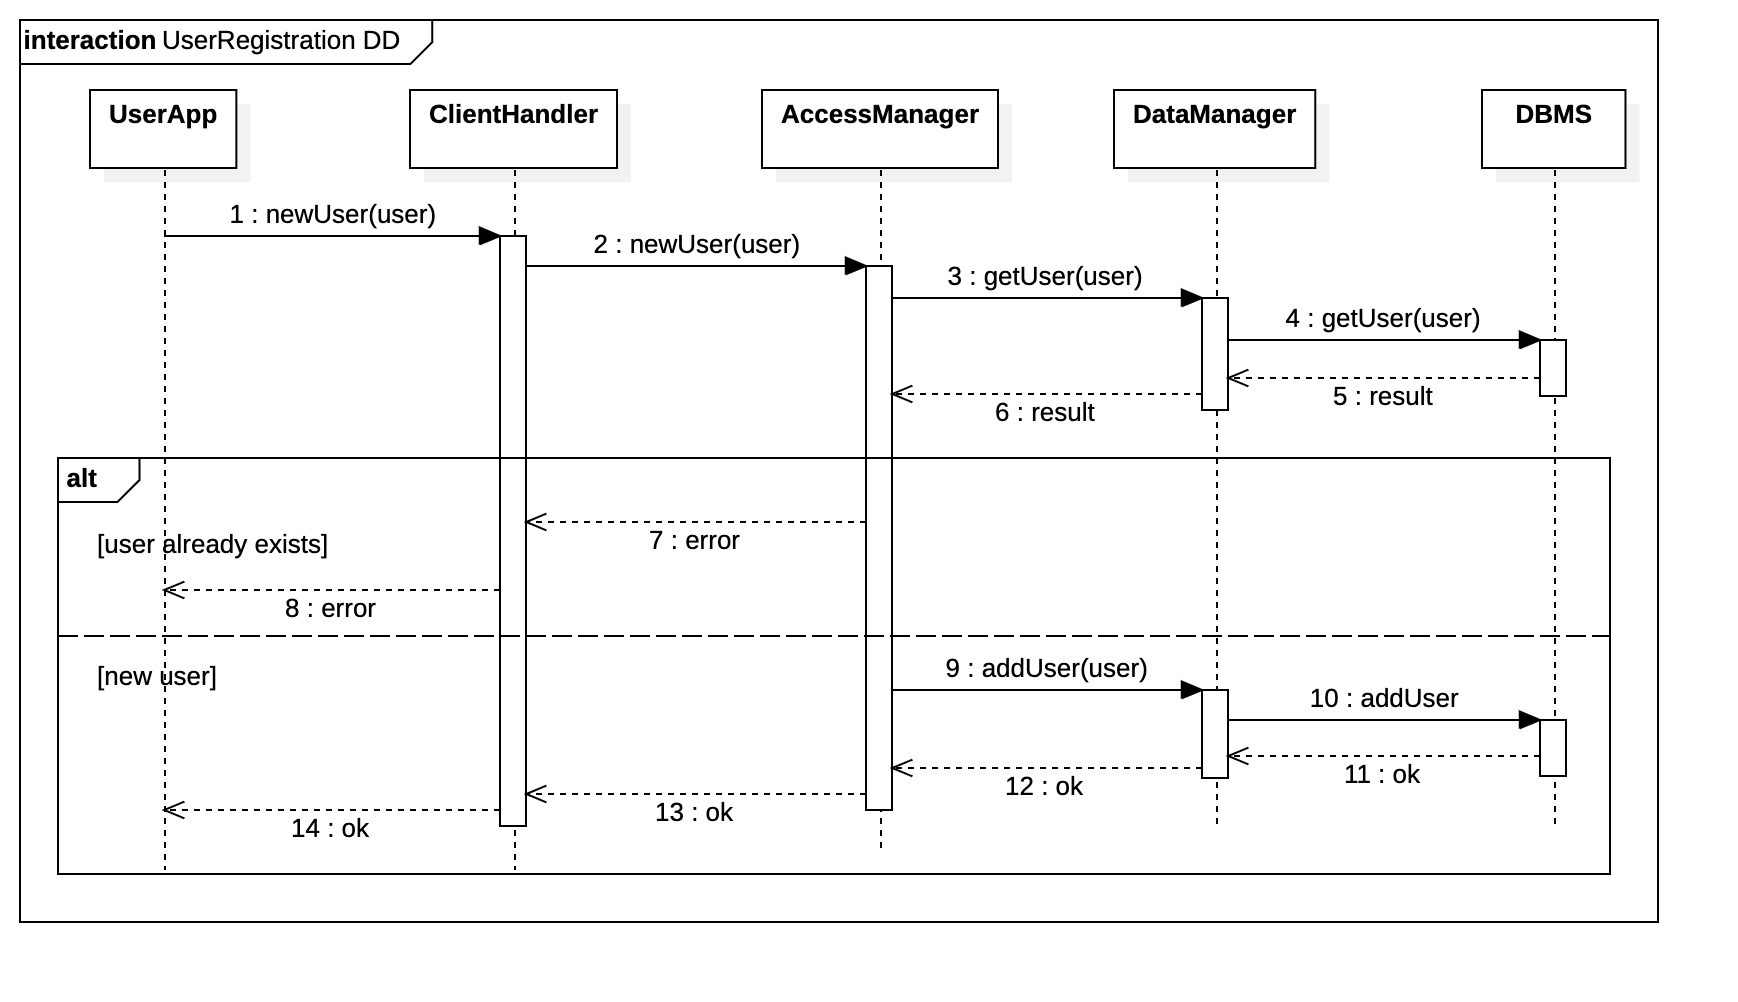
\includegraphics[scale=0.24]{/diagrams/sequence/userRegistration.png}
					\caption{User Registration sequence diagram}
				\end{figure}
				
				\FloatBarrier
			\item \textbf{User Login}
				\begin{longtable}{p{0.26\linewidth}p{0.75\linewidth}}
					\toprule
					\textbf{Name} & \textbf{User Login} \\
					\midrule
					\textbf{Actors} & User \\
					\midrule
					\textbf{Entry conditions} & The mobile application has started \\
					\midrule
					\textbf{Flow of events} & 
					\begin{enumerate}
						\item The user chooses the login option
						\item The user inserts his username
						\item The user inserts his password
						\item The user decides whether to be remembered or not
						\item The user submits the form
						\item The system checks the username to be existing
						\item The system checks the password to be right for that username
						\item The system notifies the user that login is successful
					\end{enumerate} \\
					\midrule
					\textbf{Exit conditions} & The user is logged in\\
					\midrule
					\textbf{Exceptions} & 
					\begin{itemize}
						\item If the username is not recognized by the system, that means that the user is not registered yet, or the username is incorrect. The system notifies the user and the procedure is aborted
						\item If the inserted password is wrong, the system notifies the user and the procedure is aborted			
					\end{itemize} \\
					\bottomrule
					\caption{\emph{User Login} use case description}
				\end{longtable}
			
				\begin{figure}[h]
					\centering
					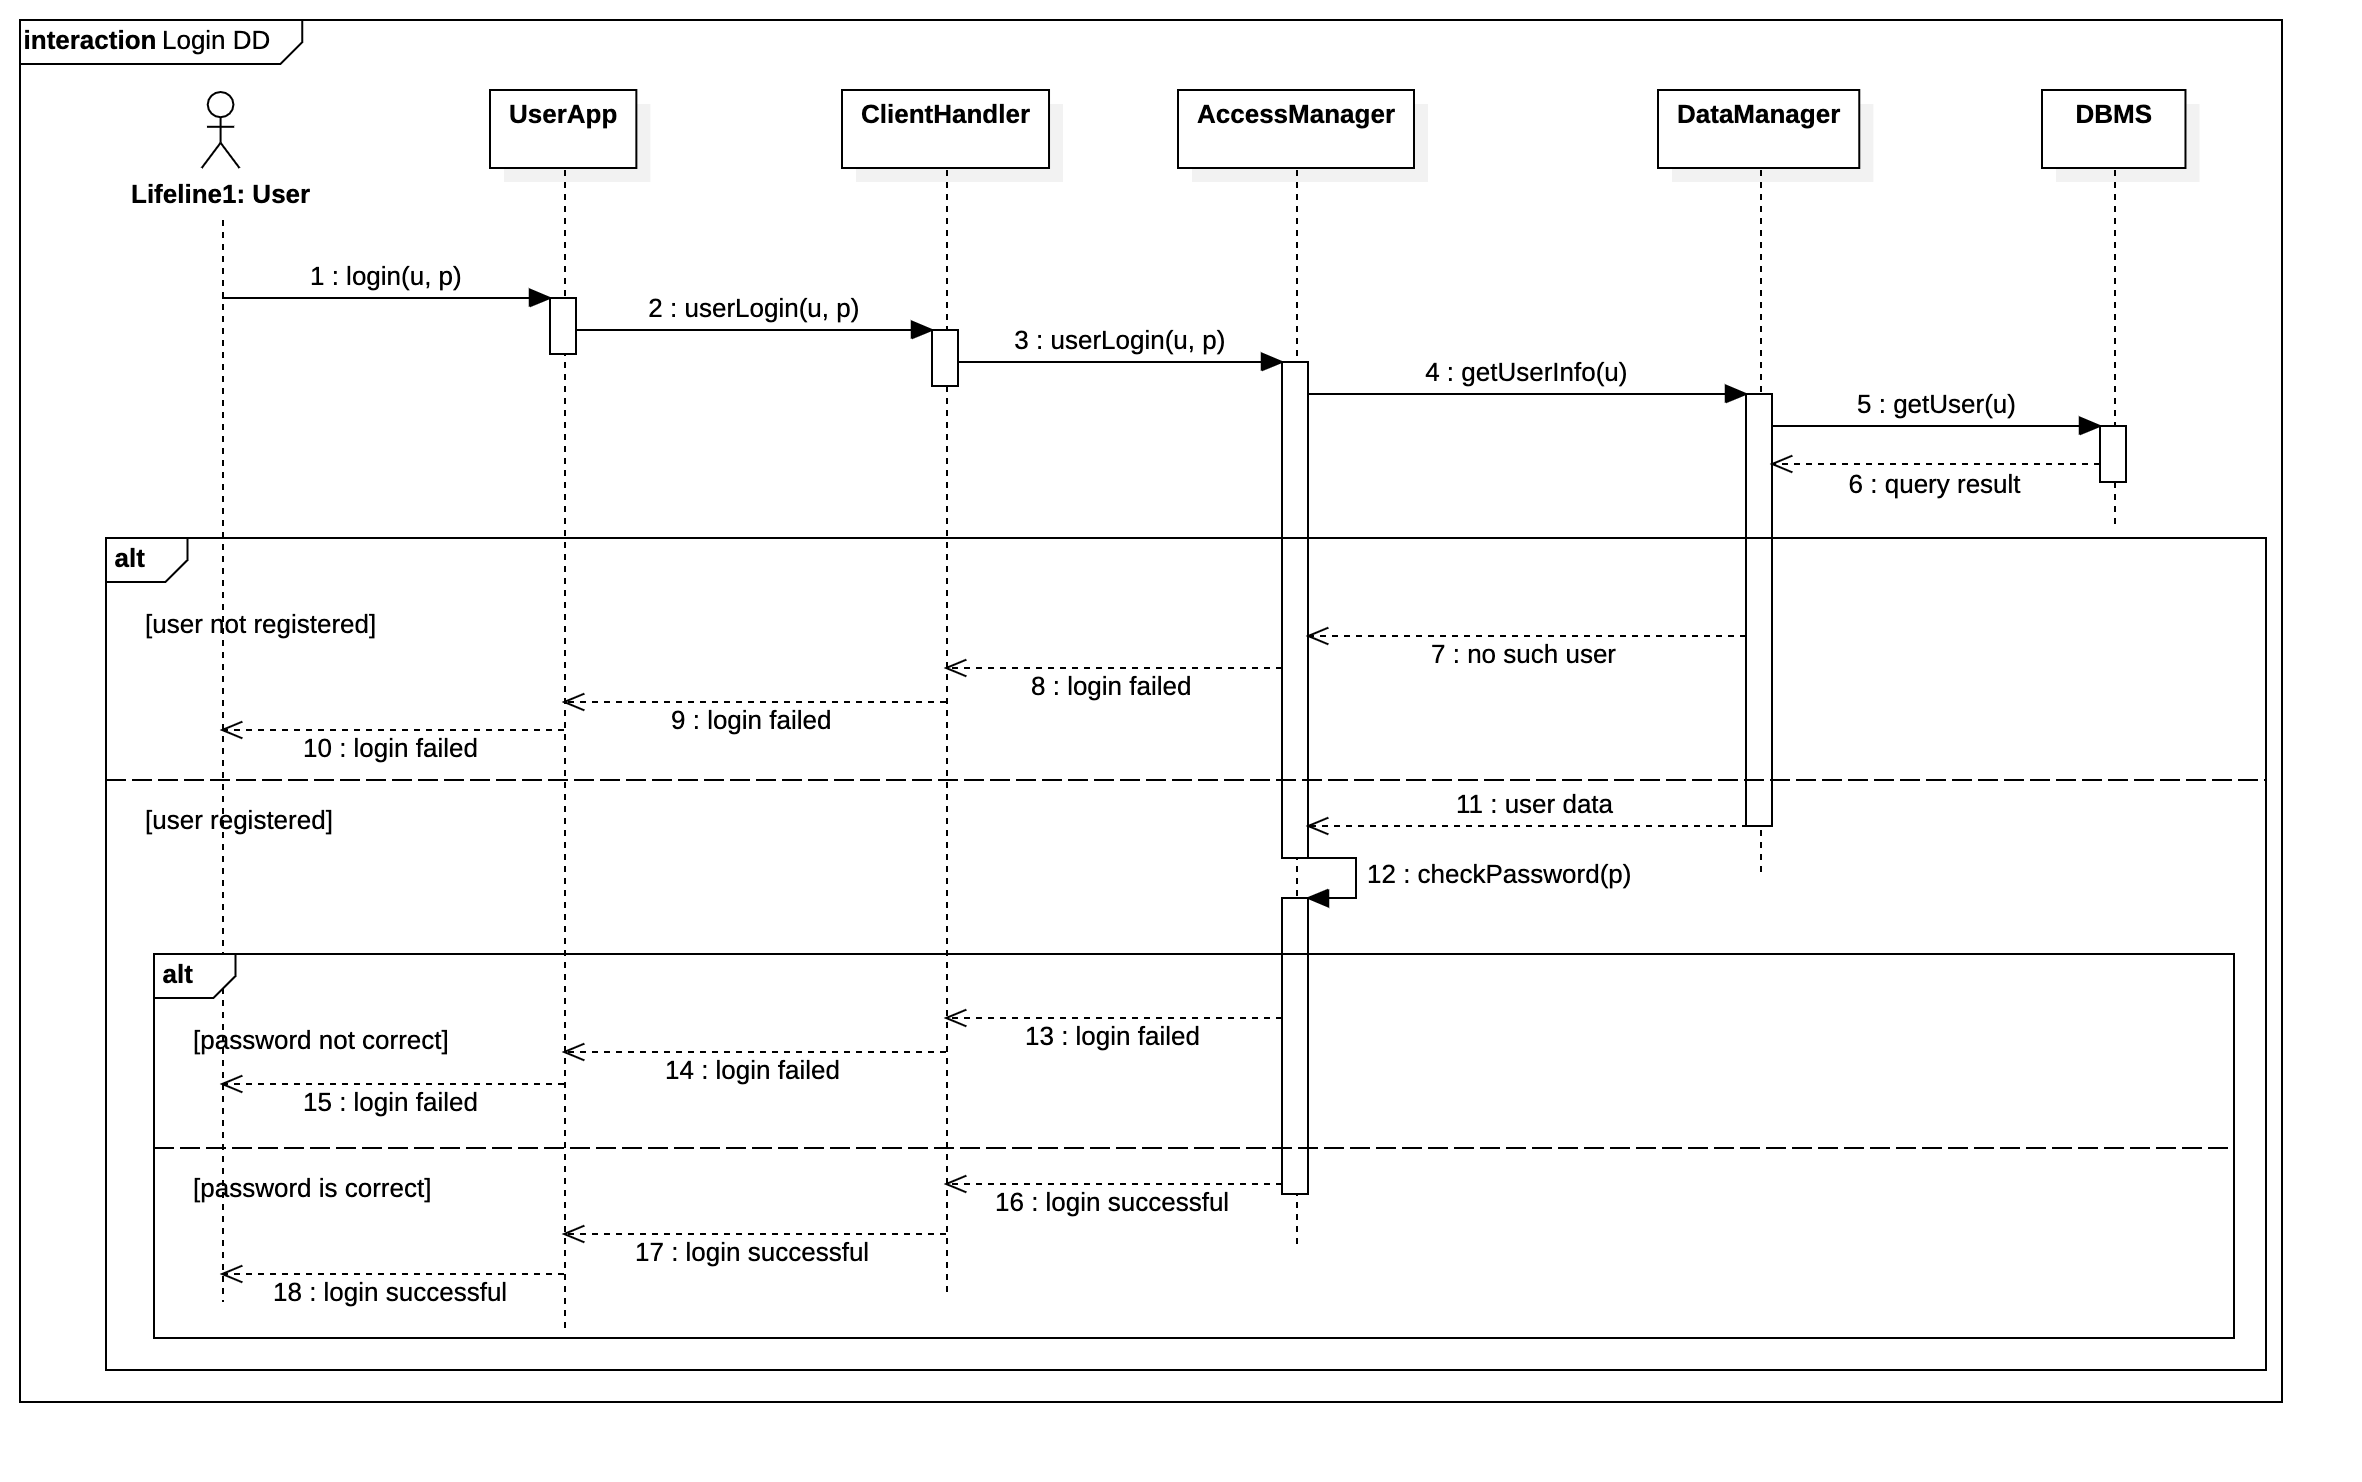
\includegraphics[scale=0.25]{/diagrams/sequence/login.png}
					\caption{User Login sequence diagram}
				\end{figure}
			
				\FloatBarrier
				\newpage
			\item \textbf{Report Violation}
				\begin{longtable}{p{0.26\linewidth}p{0.75\linewidth}}
					\toprule
					\textbf{Name} & \textbf{Report violation} \\
					\midrule
					\textbf{Actors} & User \\
					\midrule
					\textbf{Entry conditions} & The user is logged in \\
					\midrule
					\textbf{Flow of events} & 
					\begin{enumerate}
						\item The user selects the report violation option
						\item The system retrieves the GPS location
						\item The user chooses the option to take pictures
						\item The user takes some pictures through the application
						\item The user selects the pictures he wants to send
						\item The user optionally inserts the license plate number
						\item The user chooses the type of violation from a list
						\item The user chooses the type of vehicle from a list
						\item The user chooses the option to confirm
						\item The system receives the sent data
						\item The system runs an algorithm to read the license plate, with the help of the information provided by the user
						\item The system retrieves the name of the street from the GPS location
						\item The system stores the violation report
					\end{enumerate} \\
					\midrule
					\textbf{Exit conditions} & The information about the violation is stored\\
					\midrule
					\textbf{Exceptions} & 
					\begin{itemize}
						\item If the system fails to retrieve the GPS location, the user is notified and the application shows the home page
						\item If the system fails to read the license plate, or what it reads does not match the information provided by the user, the notification will be discarded
					\end{itemize} \\
					\bottomrule
					\caption{\emph{Report violation} use case description}
				\end{longtable}
			
				\begin{figure}[h]
					\centering 
					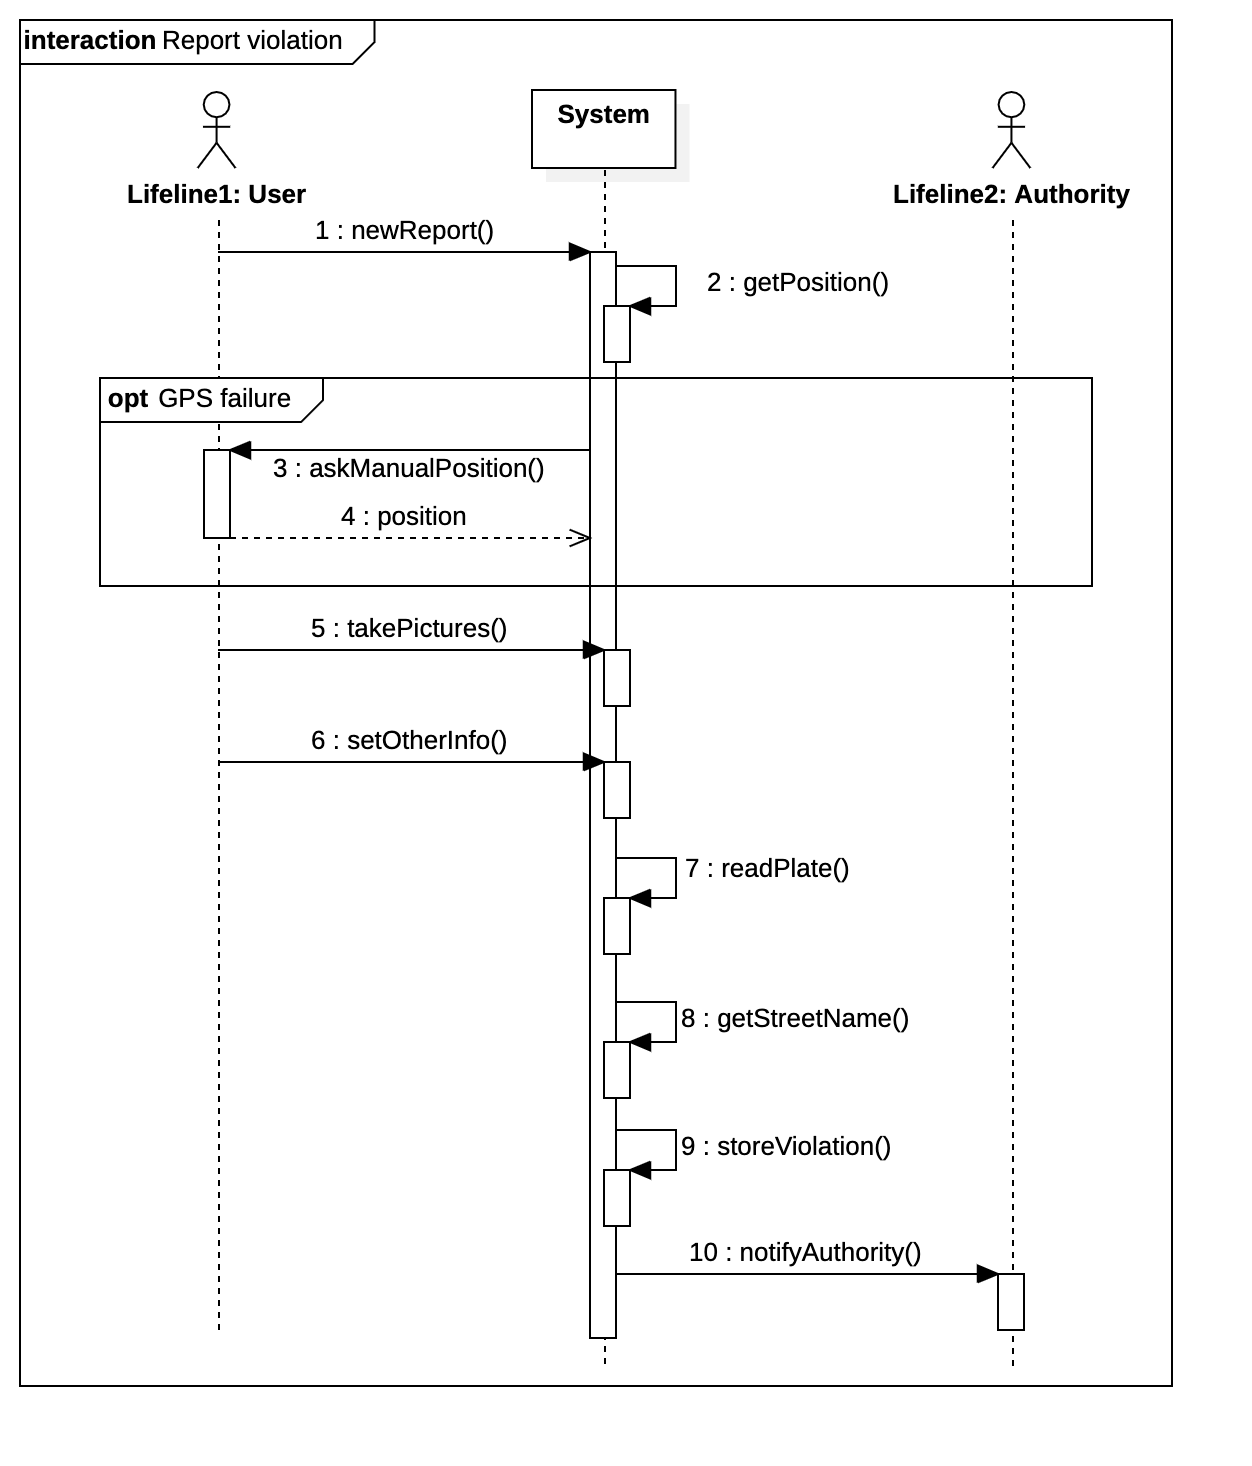
\includegraphics[scale=0.26]{/diagrams/sequence/reportViolation.png}
					\caption{Report Violation sequence diagram}
				\end{figure}
			
				\FloatBarrier
			\item \textbf{Find streets with the highest number of violations}
				\begin{longtable}{p{0.26\linewidth}p{0.75\linewidth}}
					\toprule
					\textbf{Name} & \textbf{Find streets with the highest number of violations} \\
					\midrule
					\textbf{Actors} & User \\
					\midrule
					\textbf{Entry conditions} & The user is logged in \\
					\midrule
					\textbf{Flow of events} & 
					\begin{enumerate}
						\item The user selects the 'streets with highest number of violation' option
						\item The user chooses the region he is looking for from a list
						\item The user chooses the city from a list
						\item The user chooses the types of violation to be included
						%maybe a checkbox
						\item The user chooses the time slot
						\item The user chooses the types of vehicle to be included
						\item The user confirms the query and sends it
						\item The system returns a list of the streets ordered by the highest number of violations, with the actual number next to the name of the street, according to the filters
					\end{enumerate} \\
					\midrule
					\textbf{Exit conditions} & The list of the streets is shown to the user \\
					\midrule
					\textbf{Exceptions} & 
					\begin{itemize}
						\item If no type of violation is selected, the system shows an error message and the procedure is aborted
						\item If no type of vehicle is selected, the system shows an error message and the procedure is aborted	
					\end{itemize} \\
					\bottomrule
					\caption{\emph{Find streets with the highest number of violations} use case description}
				\end{longtable}
			
				\begin{figure}[h]
					\centering
					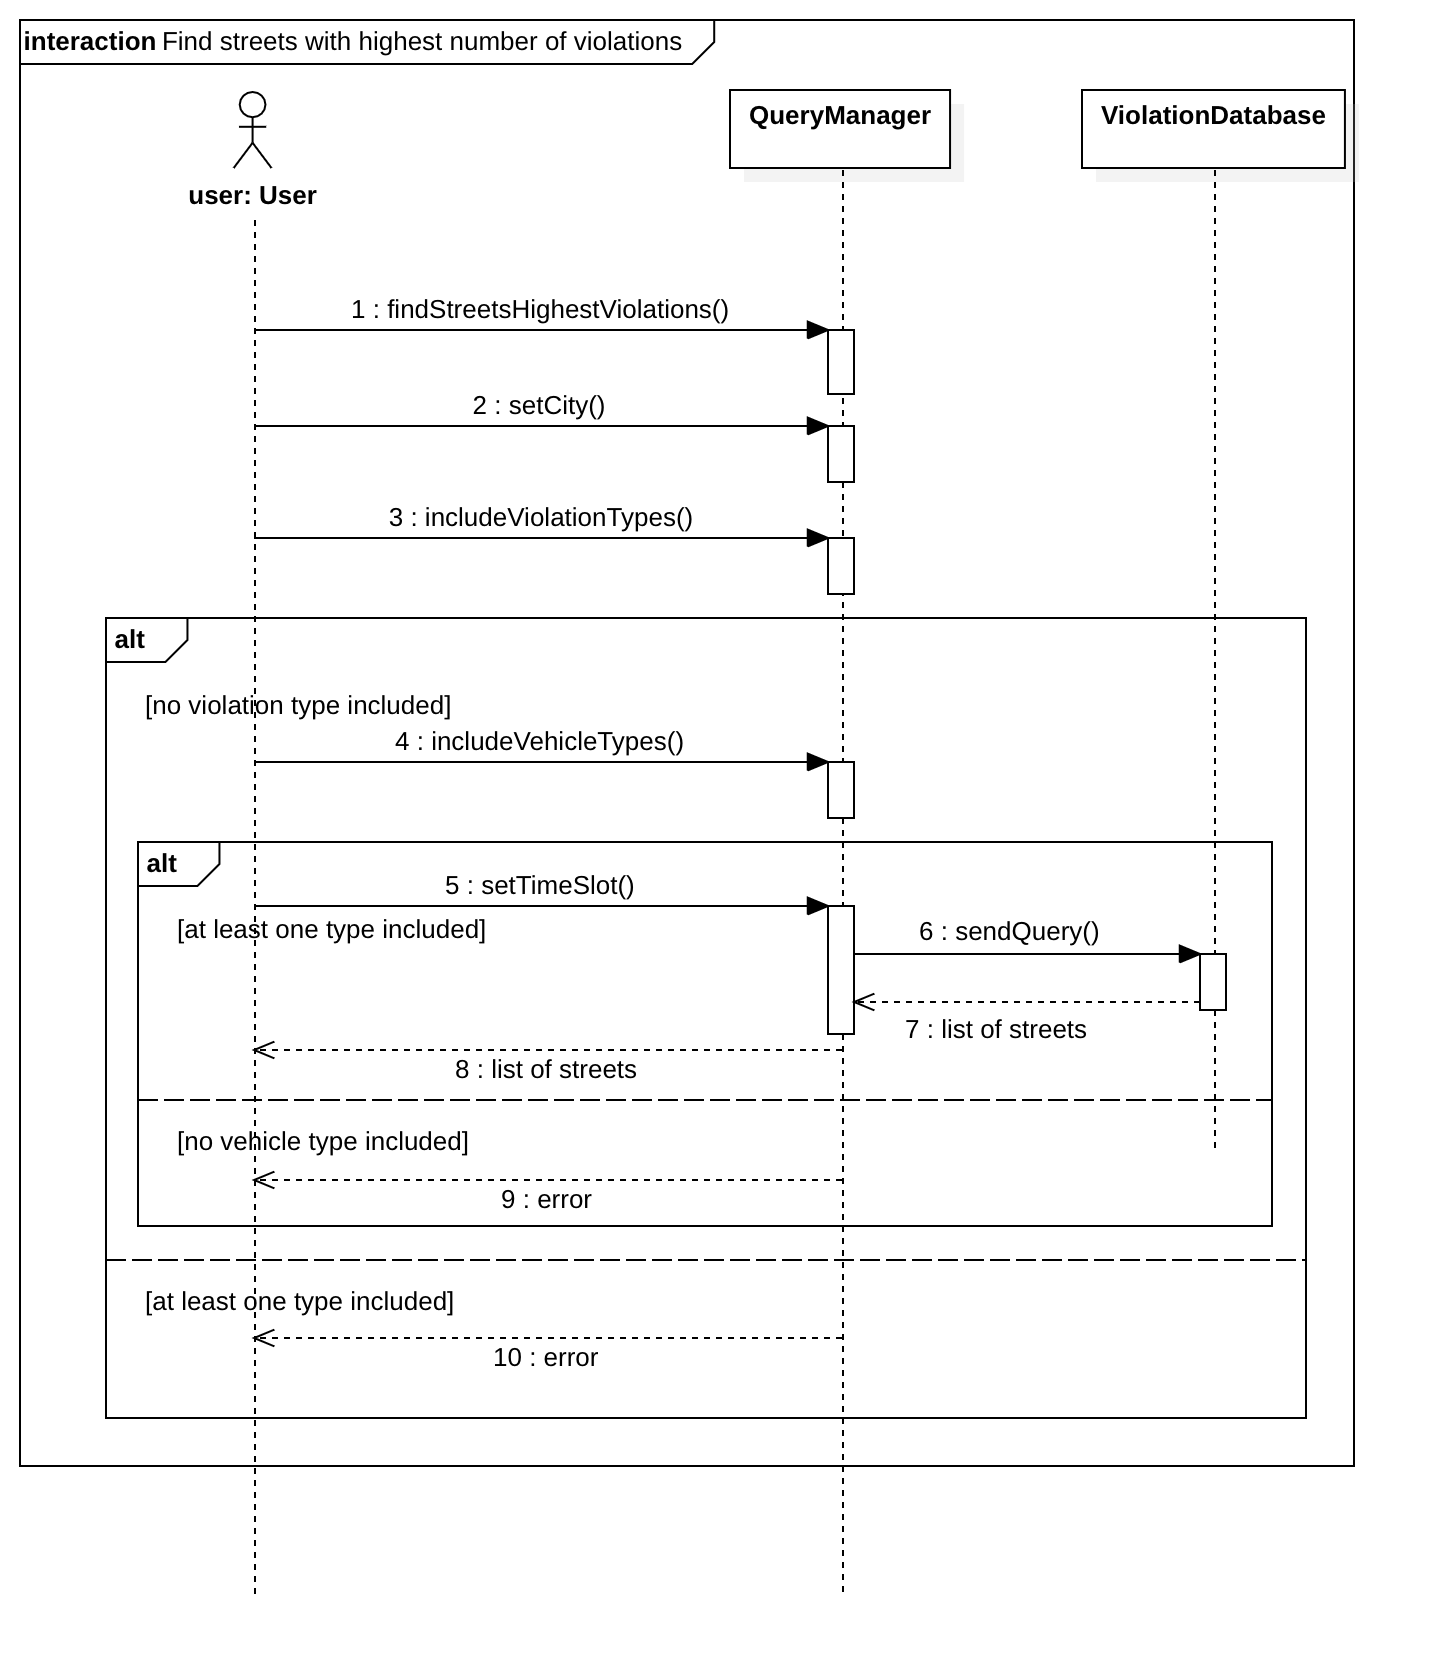
\includegraphics[scale=0.3]{/diagrams/sequence/highestViolations.png}
					\caption{Highest Number of Violations sequence diagram}
				\end{figure}
			
				\FloatBarrier
			\item \textbf{Find Most Dangerous Vehicles}
				\begin{longtable}{p{0.26\linewidth}p{0.75\linewidth}}
					\toprule
					\textbf{Name} & \textbf{Find dangerous vehicles} \\
					\midrule
					\textbf{Actors} & User \\
					\midrule
					\textbf{Entry conditions} & The user is logged in \\
					\midrule
					\textbf{Flow of events} & 
					\begin{enumerate}
						\item The user selects the 'most dangerous vehicles' option
						\item The user selects the region and the city from a list, or selects a street, or selects everywhere
						\item The user selects the types of violation he wants to include
						\item The user confirms the query and sends it
						\item The system returns a list of the types of vehicle, ordered by the highest number of violations they committed, according to the filters
					\end{enumerate} \\
					\midrule
					\textbf{Exit conditions} & The list is shown to the user\\
					\midrule
					\textbf{Exceptions} & 
					\begin{itemize}
						\item 	If no type of violation is selected, the system notifies the user and wait for him to insert at least one	
					\end{itemize} \\
					\bottomrule
					\caption{\emph{Find most dangerous vehicles} use case description}
				\end{longtable}
			
				\begin{figure}[h]
					\centering
					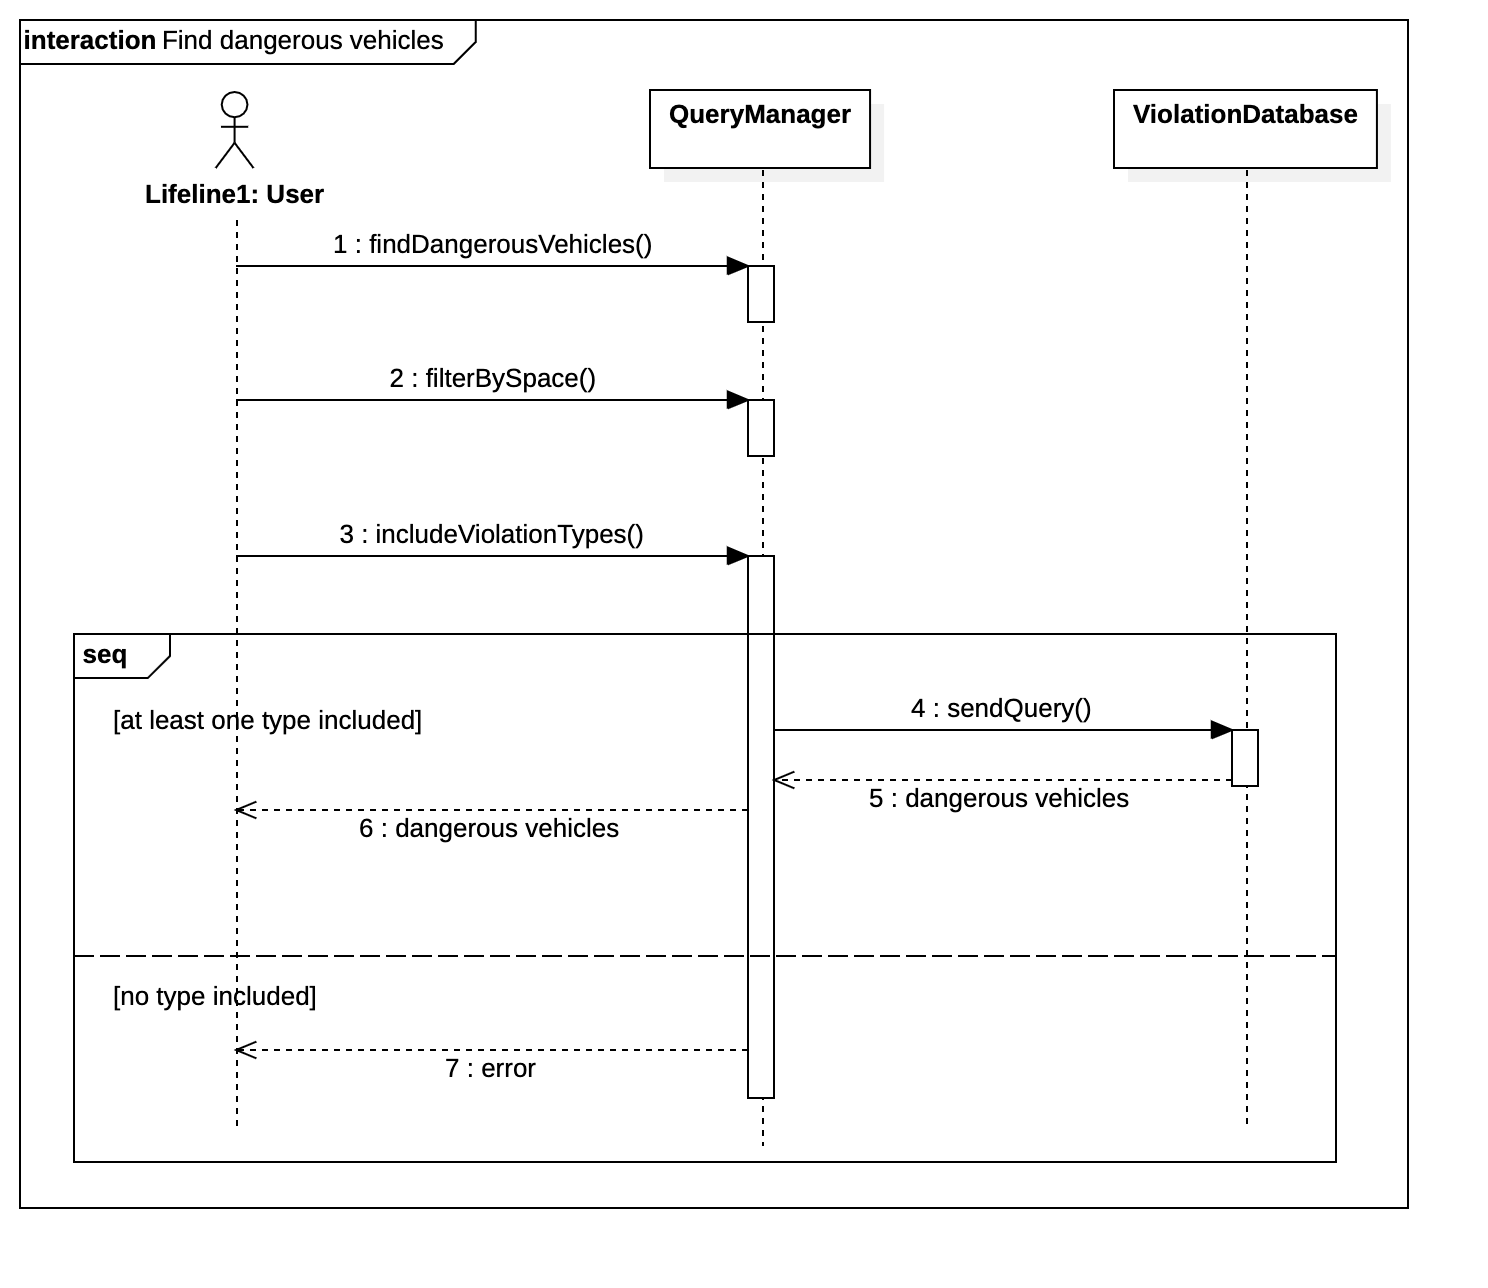
\includegraphics[scale=0.24]{/diagrams/sequence/dangerousVehicles.png}
					\caption{Dangerous Vehicles sequence diagram}
				\end{figure}
			
				\FloatBarrier
			\item \textbf{Find Urgent Interventions}
				\begin{longtable}{p{0.26\linewidth}p{0.75\linewidth}}
					\toprule
					\textbf{Name} & \textbf{Find urgent interventions} \\
					\midrule
					\textbf{Actors} & User \\
					\midrule
					\textbf{Entry conditions} & The user is logged in \\
					\midrule
					\textbf{Flow of events} & 
					\begin{enumerate}
						\item The user selects the 'urgent interventions' option
						\item The user selects the region and the city from a list
						\item The user confirms the query and sends it
						\item The system returns a list of the most urgent interventions in the selected city, each with their respective street
					\end{enumerate} \\
					\midrule
					\textbf{Exit conditions} & The list is shown to the user\\
					\midrule
					\textbf{Exceptions} &  \\
					\bottomrule
					\caption{\emph{Find urgent interventions} use case description}
				\end{longtable}
			
				\newpage
			
				\begin{figure}[hbtp]
					\centering
					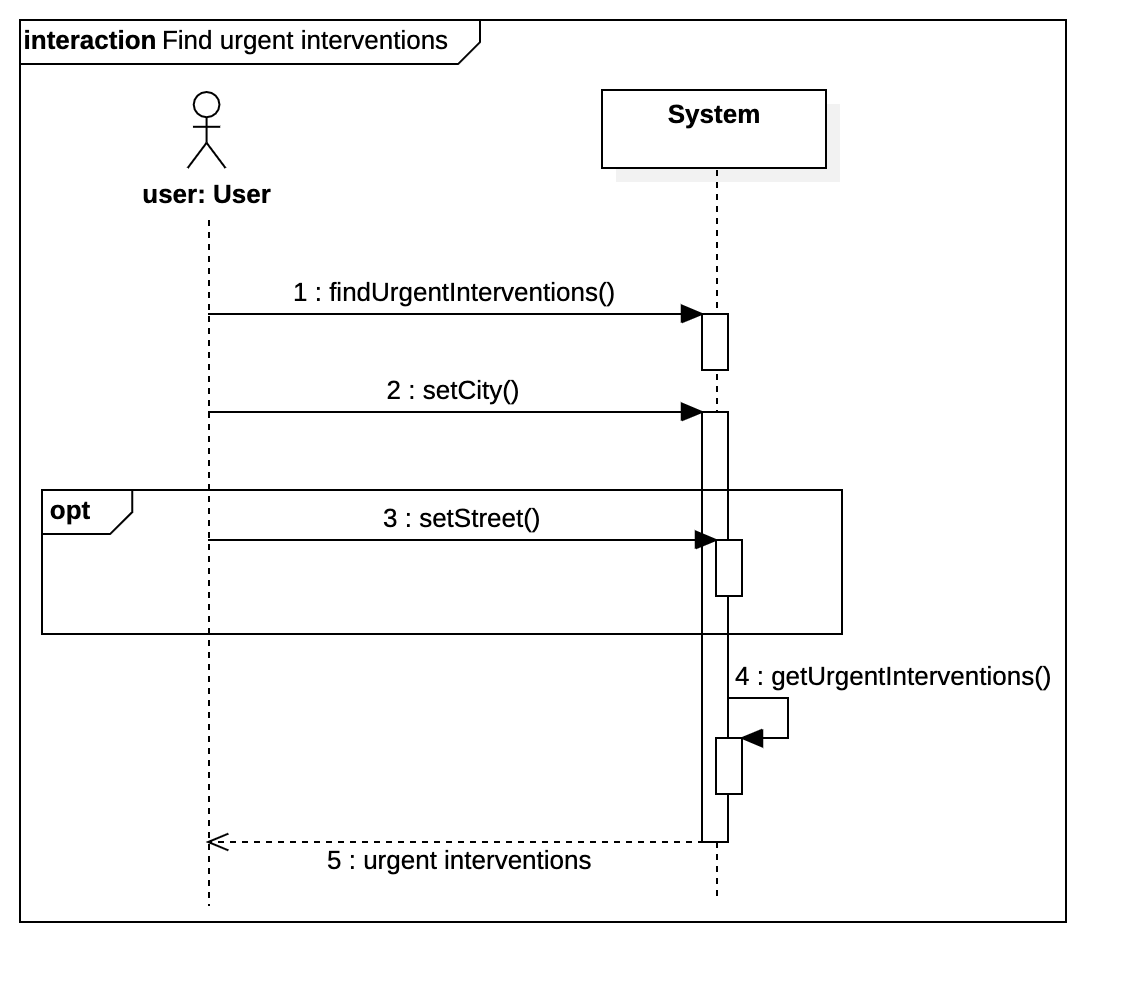
\includegraphics[scale=0.28]{/diagrams/sequence/urgentInterventions.png}
					\caption{Urgent Interventions sequence diagram}
				\end{figure}
			
				\FloatBarrier
			\item \textbf{Find Unsafe Streets}
				\begin{longtable}{p{0.26\linewidth}p{0.75\linewidth}}
					\toprule
					\textbf{Name} & \textbf{Find unsafe streets} \\
					\midrule
					\textbf{Actors} & User \\
					\midrule
					\textbf{Entry conditions} & The user is logged in \\
					\midrule
					\textbf{Flow of events} & 
					\begin{enumerate}
						\item The user selects the 'unsafe streets' option
						\item The user selects the either the 'city' option, the 'route' option or the single street option
						\item The user chooses the region and the city from a list if 'city' option is chosen, if 'route' option is chosen he enters start and end points of the route, otherwise he inserts the name of the street
						\item The user confirms the query and sends it
						\item The system returns a map where the streets selected with the filter are colored according to their safety: green if they're 'safe', red if they're 'unsafe'
					\end{enumerate} \\
					\midrule
					\textbf{Exit conditions} & The list is shown to the user\\
					\midrule
					\textbf{Exceptions} & 
					\begin{itemize}
						\item If no city is selected when 'city' option is chosen, the system notifies the user and waits for him to insert it
						\item If no start or end points are chosen when 'route' option is selected, the system notifies the user and waits for him to insert them
					\end{itemize} \\
					\bottomrule
					\caption{\emph{Find unsafe streets} use case description}
				\end{longtable}
		\end{enumerate}
		
		\begin{figure}[h!]
			\centering
			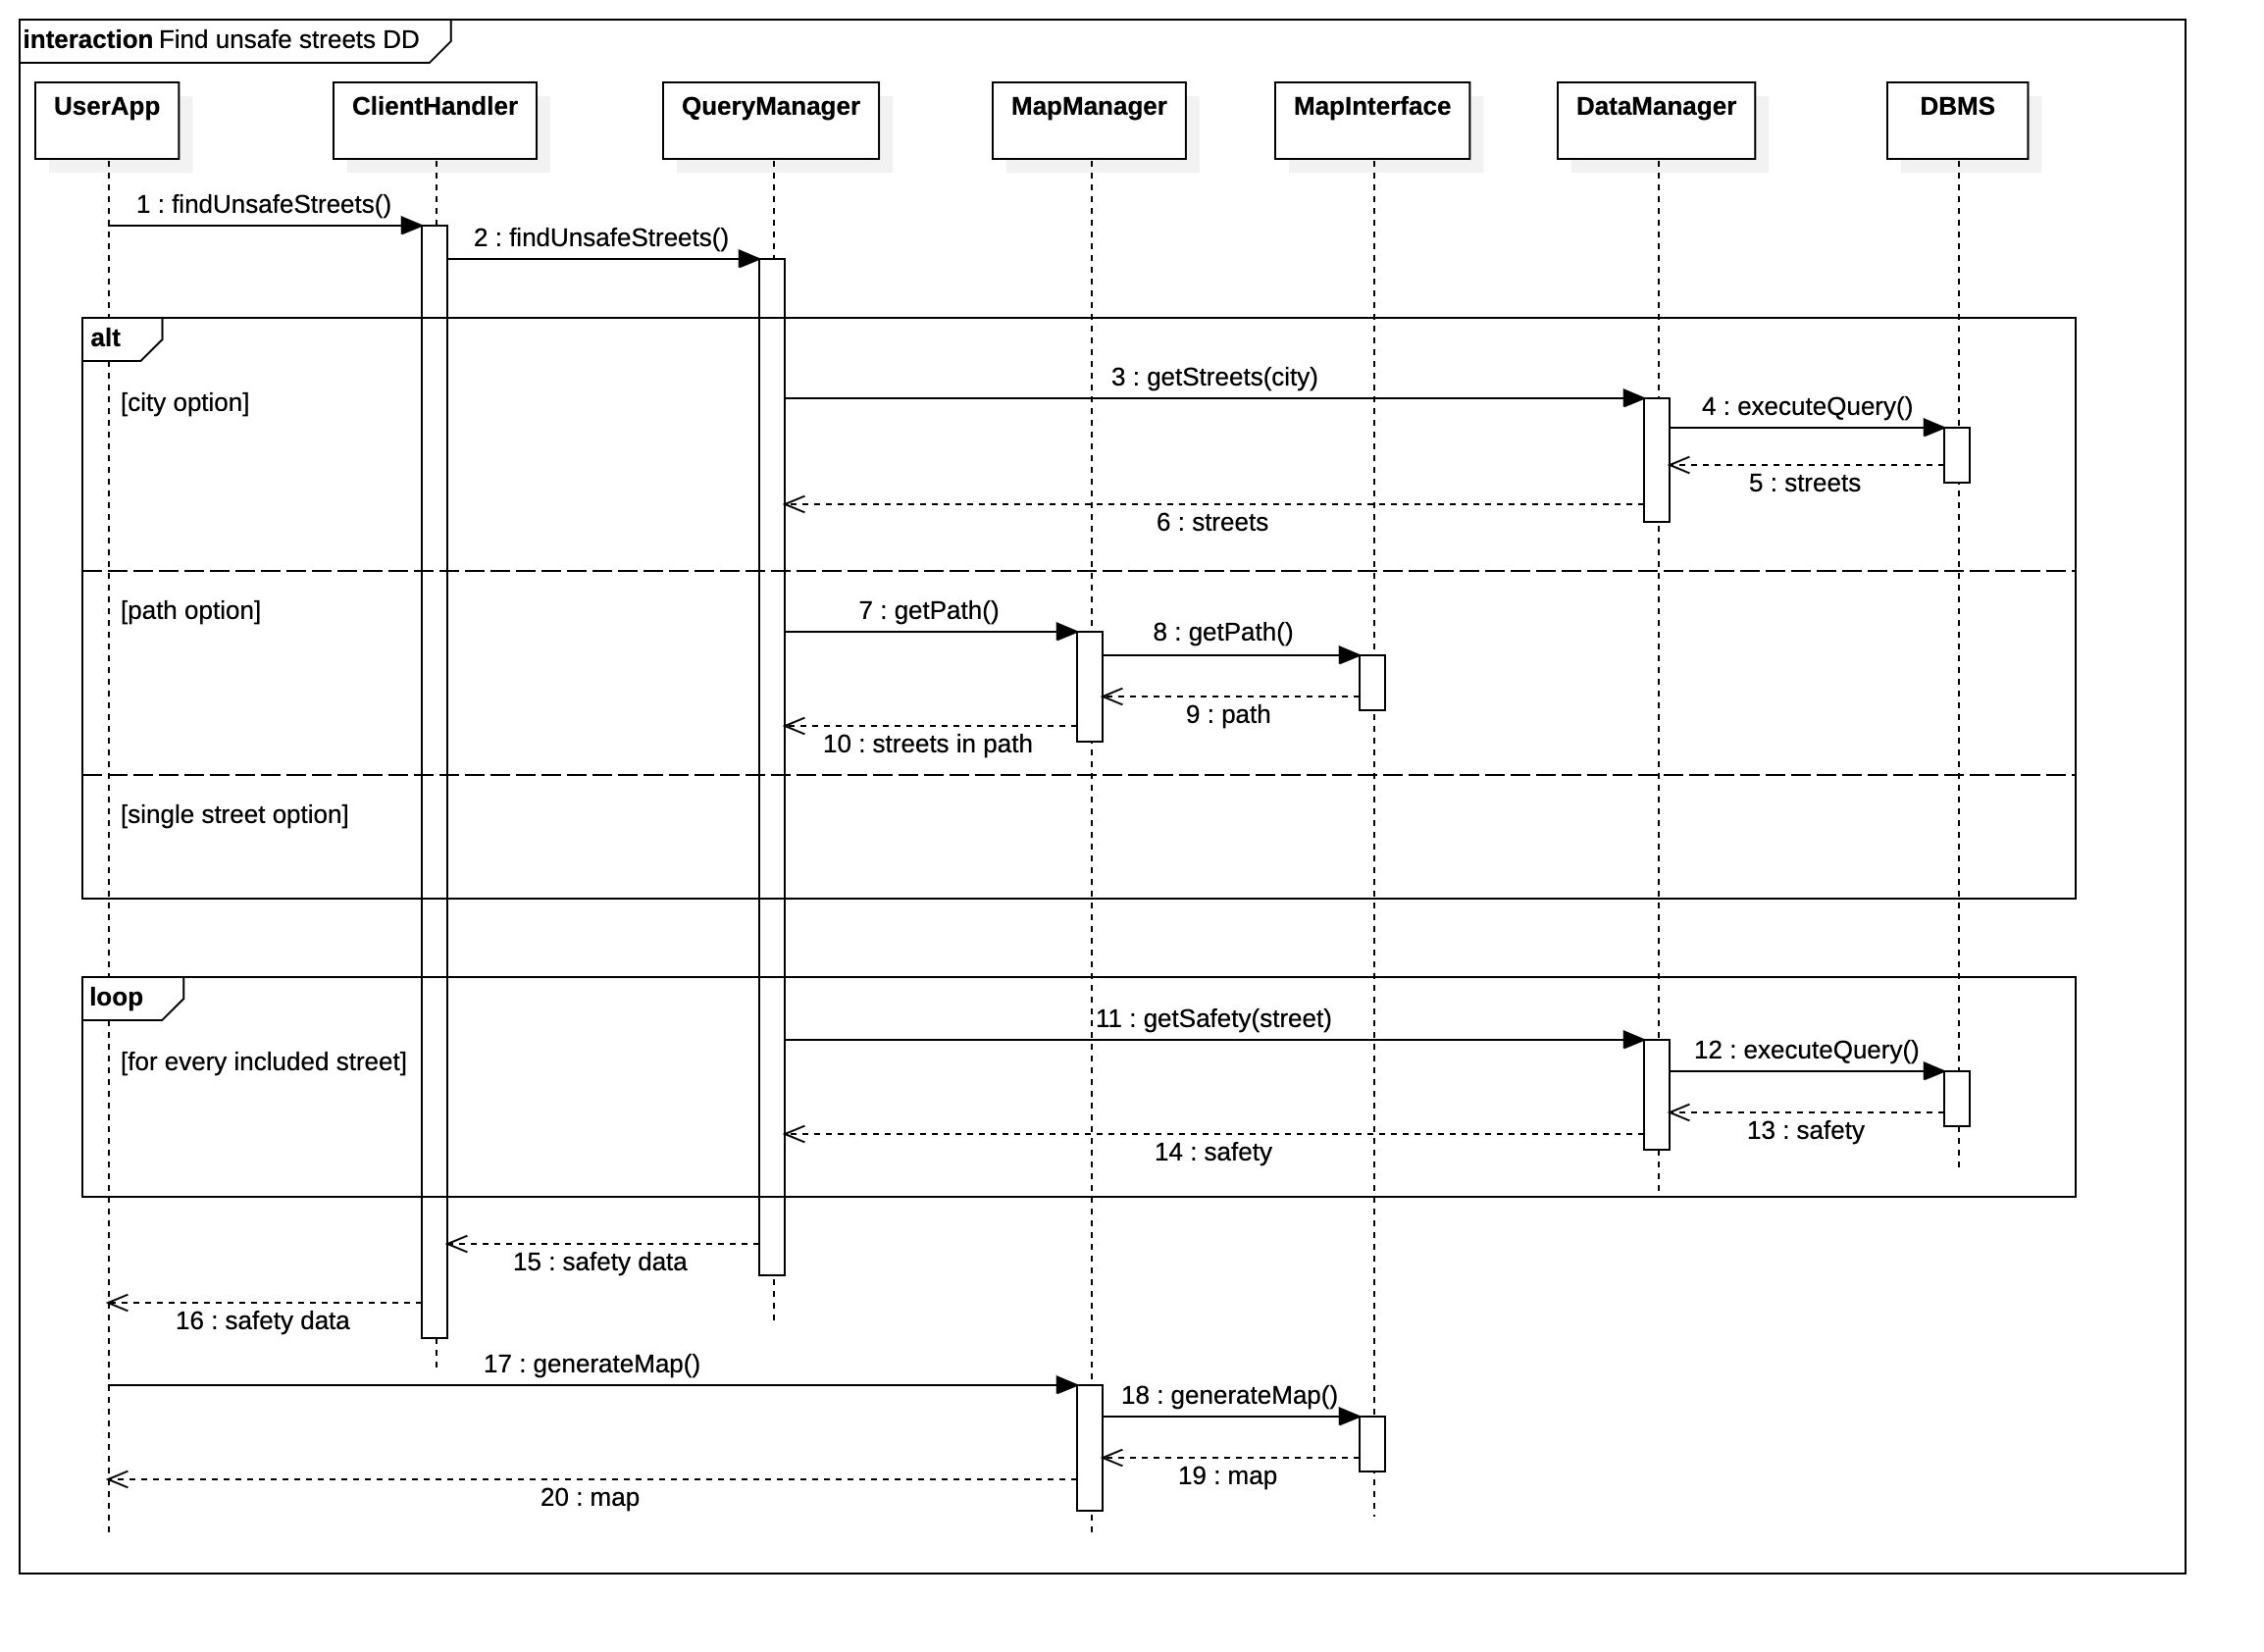
\includegraphics[scale=0.28]{/diagrams/sequence/unsafeStreets.png}
			\caption{Unsafe Streets sequence diagram}
		\end{figure}
			
		\FloatBarrier
		\newpage
			
		\paragraph{Authority}
		\begin{enumerate}
			\item \textbf{Authority Registration}
				\begin{longtable}{p{0.26\linewidth}p{0.75\linewidth}}
					\toprule
					\textbf{Name} & \textbf{Registration} \\
					\midrule
					\textbf{Actors} & Authority \\
					\midrule
					\textbf{Entry conditions} & The web application has started \\
					\midrule
					\textbf{Flow of events} & 
					\begin{enumerate}
						\item The authority chooses the sign up option
						\item The authority chooses the region and the city of competence
						\item The authority inserts its PEC address
						\item The system checks that PEC address matches the chosen city
						\item The system sends a confirmation code to the PEC address
						\item The authority enters the confirmation code in a text box
						\item The authority chooses the password
						\item The authority accepts the \emph{Terms and Conditions} of SafeStreets
						\item The authority submits the form
						\item The system checks the entered code to match the sent one
						\item The system saves the authority's data
					\end{enumerate} \\
					\midrule
					\textbf{Exit conditions} & The authority is registered in the system\\
					\midrule
					\textbf{Exceptions} & 
					\begin{itemize}
						\item If the selected city already has an authority registered, an error message is shown and the procedure is aborted
						\item If the PEC address doesn't match the chosen city, an error message is shown and the procedure is aborted
						\item If the entered code doesn't match the sent one, an error message is shown and the procedure is aborted
					\end{itemize} \\
					\bottomrule
					\caption{\emph{Authority Registration} use case description}
				\end{longtable}
			
				\begin{figure}[h]
					\centering
					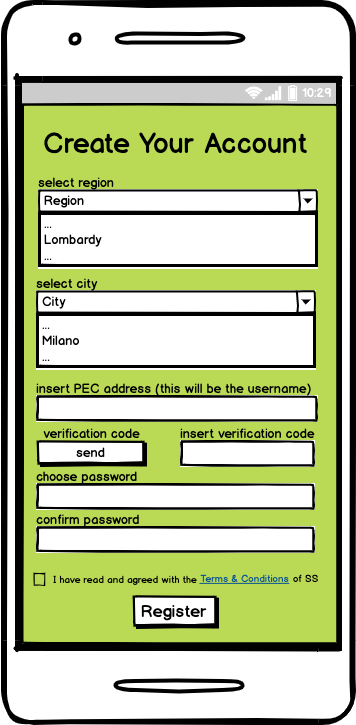
\includegraphics[scale=0.25]{/diagrams/sequence/authorityRegistration.png}
					\caption{Authority Registration sequence diagram}
				\end{figure}
			
				\FloatBarrier
			\item \textbf{Authority Login}
				\begin{longtable}{p{0.26\linewidth}p{0.75\linewidth}}
					\toprule
					\textbf{Name} & \textbf{Authority Login} \\
					\midrule
					\textbf{Actors} & Authority\\
					\midrule
					\textbf{Entry conditions} & The web application has started \\
					\midrule
					\textbf{Flow of events} & 
					\begin{enumerate}
						\item The authority chooses the login option
						\item The authority chooses the 'authority' login type
						\item The authority inserts its PEC address as username
						\item The authority inserts its password
						\item The authority decides whether to be remembered or not
						\item The authority submits the form
						\item The system checks the username to be registered
						\item The system checks the password to be right for that username
						\item The system notifies the authority that login is successful
					\end{enumerate} \\
					\midrule
					\textbf{Exit conditions} & The authority is logged in\\
					\midrule
					\textbf{Exceptions} & 
					\begin{itemize}
						\item If the username is not recognized by the system, that means that the authority is not registered yet, or the username is incorrect. The system notifies the authority and the procedure is aborted
						\item If the inserted password is wrong, the system notifies the authority and the procedure is aborted			
					\end{itemize} \\
					\bottomrule
					\caption{\emph{Authority Login} use case description}
				\end{longtable}
			
			\item \textbf{Check Unread Reports}
				\begin{longtable}{p{0.26\linewidth}p{0.75\linewidth}}
					\toprule
					\textbf{Name} & \textbf{Check unread reports} \\
					\midrule
					\textbf{Actors} & Authority\\
					\midrule
					\textbf{Entry conditions} & The authority is logged in \\
					\midrule
					\textbf{Flow of events} & 
					\begin{enumerate}
						\item The authority chooses the 'unread reports' option
						\item The system provides a list with all the unread violation reports that match the city of competence of the authority
					\end{enumerate} \\
					\midrule
					\textbf{Exit conditions} & The list is shown to the authority\\
					\midrule
					\textbf{Exceptions} &  \\
					\bottomrule
					\caption{\emph{Check unread reports} use case description}
				\end{longtable}
				
				\begin{figure}[h]
					\centering
					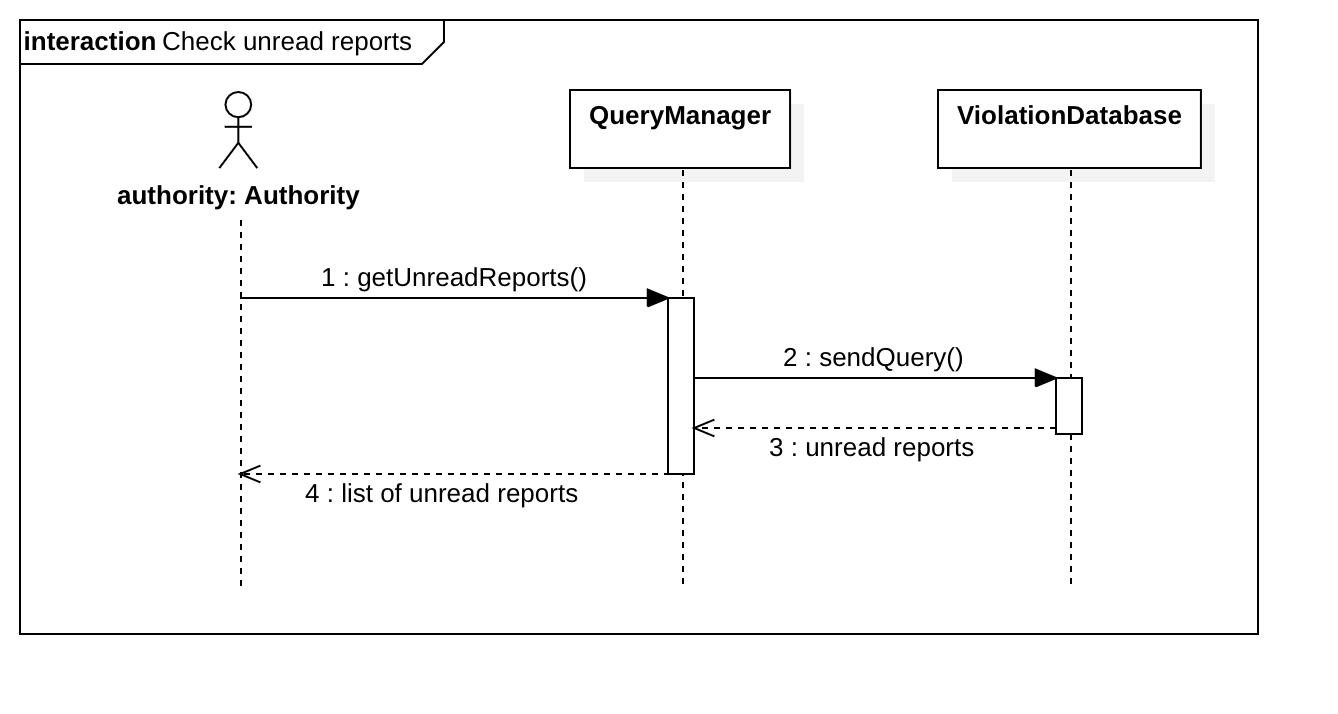
\includegraphics[scale=0.34]{/diagrams/sequence/unreadReports.png}
					\caption{Unread Reports sequence diagram}
				\end{figure}
				
				\FloatBarrier
				\newpage
			\item \textbf{Find Reports}
				\begin{longtable}{p{0.26\linewidth}p{0.75\linewidth}}
					\toprule
					\textbf{Name} & \textbf{Find reports} \\
					\midrule
					\textbf{Actors} & Authority\\
					\midrule
					\textbf{Entry conditions} & The authority is logged in \\
					\midrule
					\textbf{Flow of events} & 
					\begin{enumerate}
						\item The authority chooses the 'find reports' option
						\item The authority selects the types of violation to be included
						\item The authority selects date interval and time slot
						\item The authority selects the types of vehicle to be included
						\item The authority optionally selects the street to include, otherwise 'city' will be selected
						\item The authority confirms and sends the query
						\item The system provides a list with all the violation reports that match the filter, sorted by chronological order from the most recent one. In case 'city' option is selected, the considered city is that of competence of the authority
					\end{enumerate} \\
					\midrule
					\textbf{Exit conditions} & The list is shown to the authority\\
					\midrule
					\textbf{Exceptions} &  
					\begin{enumerate}
						\item If the date interval is not valid, the system notifies the authority and the procedure is aborted
					\end{enumerate}\\
					\bottomrule
					\caption{\emph{Find reports} use case description}
				\end{longtable}
	
				\begin{figure}[hbtp]
					\centering
					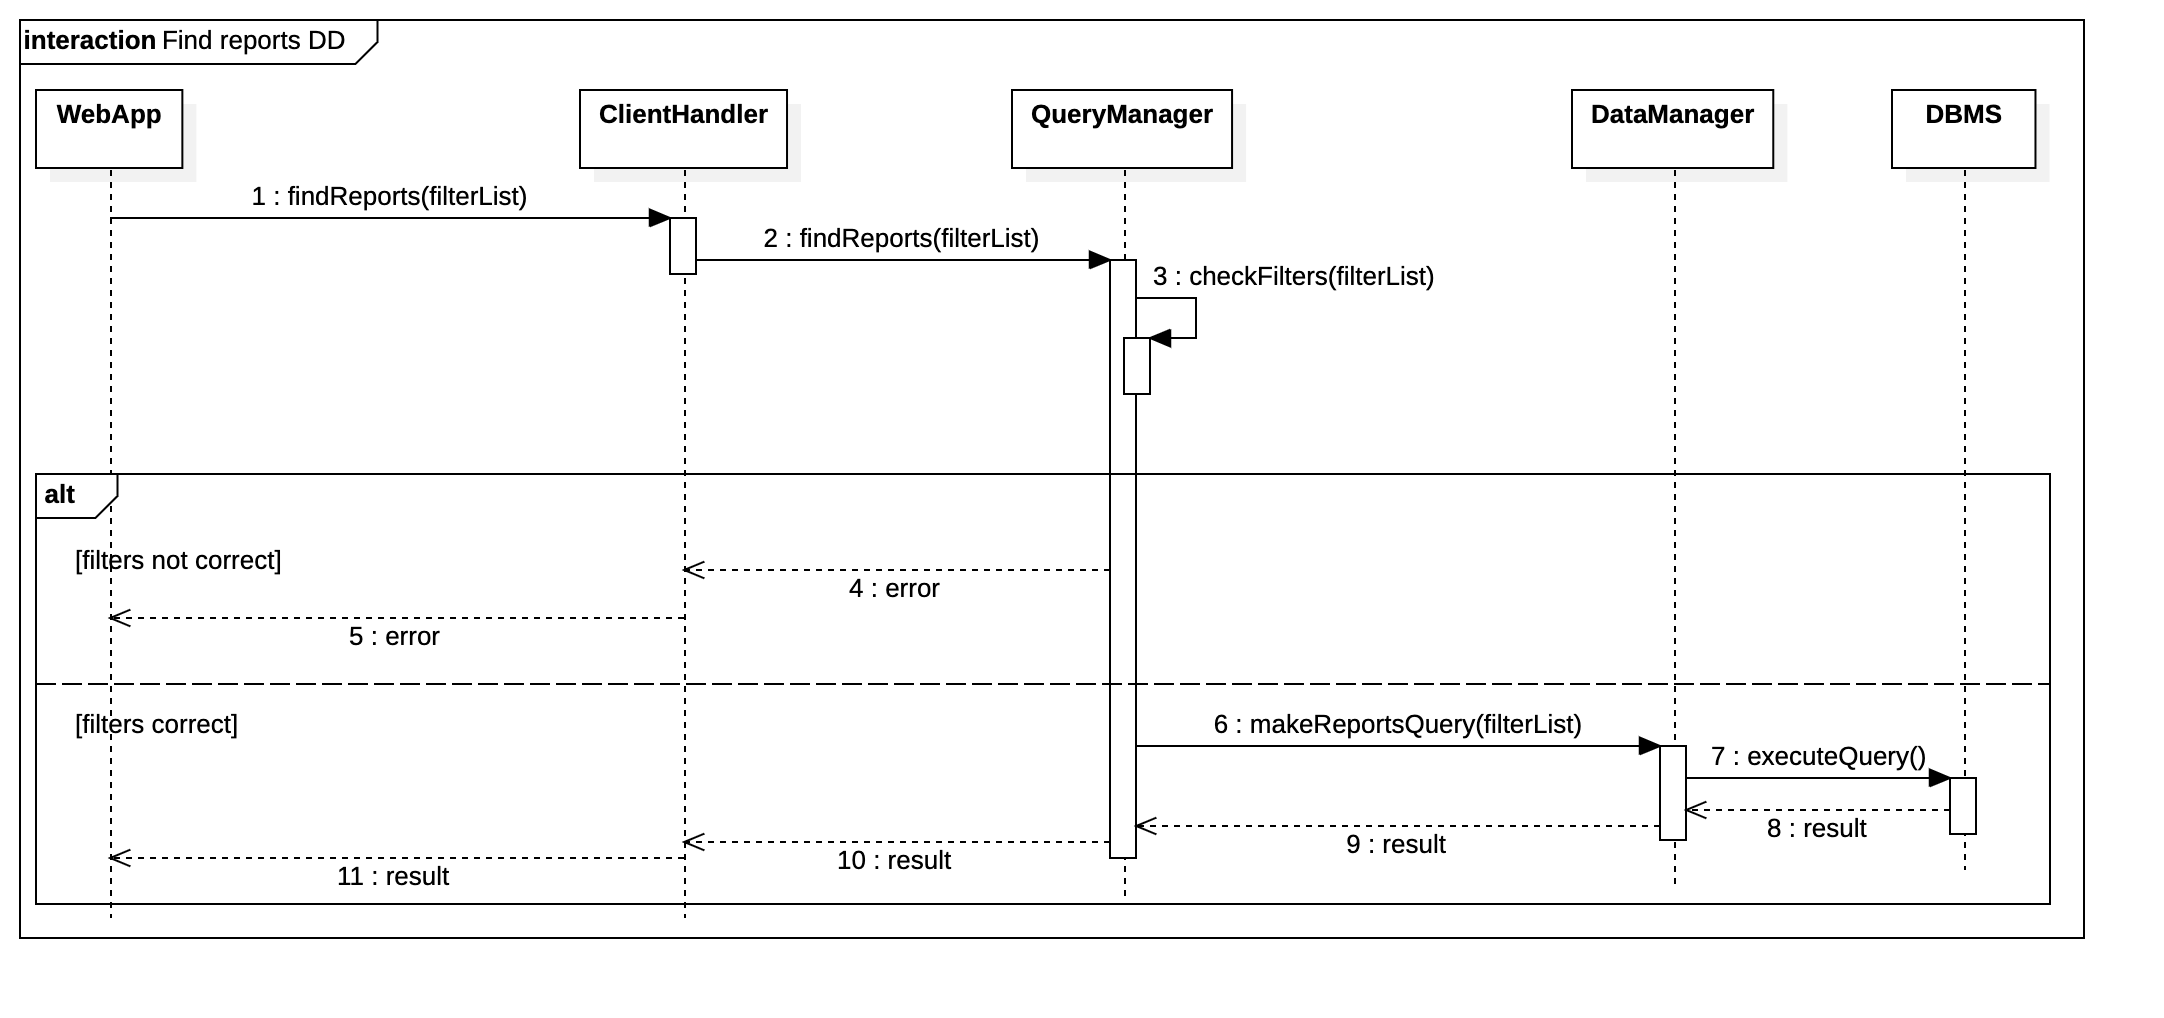
\includegraphics[scale=0.31]{/diagrams/sequence/findReports.png}
					\caption{Find Reports sequence diagram}
				\end{figure}
		\end{enumerate}

	\FloatBarrier

	\subsubsection[Traceability Matrix]{\hyperlink{toc}{Traceability Matrix}}
		\label{tab:traceabilityMatrix}
		
		\begin{table}[h!]
			\centering
			\begin{minipage}{0.5\textheight}
				\centering
				\begin{tabular}{|c|c|c|c|c|c|c|c|c|c|c|}
					\cline{2-11}
					\multicolumn{1}{c|}{} & \blueRef{req:userReg} & \blueRef{req:authorityReg} & \blueRef{req:userLogin} & \blueRef{req:authorityLogin} & \blueRef{req:uniqueName} & \blueRef{req:saveRegData} & \blueRef{req:specialCharacters} & \blueRef{req:takePictures} & \blueRef{req:dateTime}  & \blueRef{req:gpsPosition}\\
					\hline
					Registration & \xmark & \xmark & & & \xmark & \xmark & \xmark & & &\\
					\hline
					Login & & & \xmark & \xmark & \xmark & & \xmark & & &\\
					\hline
					Report Violation & \xmark & & \xmark & & & & \xmark & \xmark & \xmark & \xmark \\
					\hline
					Highest Violations & \xmark & \xmark & \xmark & \xmark & & & & & &\\
					\hline
					Dangerous Vehicles & \xmark & \xmark & \xmark & \xmark & & & & & &\\
					\hline
					Urgent Interventions & \xmark & \xmark & \xmark & \xmark & & & & & &\\
					\hline
					Unsafe Streets & \xmark & \xmark & \xmark & \xmark & & & & & &\\
					\hline
					Unread Reports & & \xmark & & \xmark & & & & & &\\
					\hline
					Find Reports & & \xmark & & \xmark & & & & & &\\
					\hline
					\blueRef{sce:notification} & \xmark & & \xmark & & & & \xmark & \xmark & \xmark & \xmark \\
					\hline
					\blueRef{sce:basicUser} & \xmark & & \xmark & & & & & & &\\
					\hline
					\blueRef{sce:advancedUser} & \xmark & & \xmark & & & & & & &\\
					\hline
					\blueRef{sce:findReports} & & \xmark & & \xmark & & & & & &\\
					\hline
					\blueRef{sce:basicAuthority} & & \xmark & & \xmark & & & & & &\\
					\hline
					\blueRef{sce:advancedAuthority} & & \xmark & & \xmark & & & & & &\\
					\hline
				\end{tabular}
				\vspace{0.4cm}
				\caption{Requirements from R1 to R10}
			\end{minipage}
		\end{table}
		
		\vfill
		
		\begin{table}[h!]
			\centering
			\begin{minipage}{0.5\textheight}
				\begin{tabular}{|c|c|c|c|c|c|c|c|c|c|}
					\cline{2-10}
					\multicolumn{1}{c|}{} & \blueRef{req:violationType} &  \blueRef{req:vehicleType} & \blueRef{req:plateNumber} & \blueRef{req:readPlate} & \blueRef{req:storeViolation} & \blueRef{req:streetName} & \blueRef{req:notifyAuthority} & \blueRef{req:mineData} & \blueRef{req:cityFilter} \\
					\hline
					Registration & & & & & & & & & \\
					\hline
					Login & & & & & & & & & \\
					\hline
					Report Violation & \xmark & \xmark & \xmark & \xmark & \xmark & \xmark & \xmark & \xmark & \\
					\hline
					Highest Violations & & & & & & & & \xmark & \xmark \\
					\hline
					Dangerous Vehicles & & & & & & & & \xmark & \xmark \\
					\hline
					Urgent Interventions & & & & & \xmark & & & & \xmark \\
					\hline
					Unsafe Streets & & & & & \xmark & & & & \xmark\\
					\hline
					Unread Reports & & & & & \xmark & & & & \\
					\hline
					Find Reports & & & & & \xmark & & & & \xmark \\
					\hline
					\blueRef{sce:notification} & \xmark & \xmark & \xmark & \xmark & \xmark & \xmark & \xmark & \xmark &\\
					\hline
					\blueRef{sce:basicUser} & & & & & & & & \xmark & \xmark\\
					\hline
					\blueRef{sce:advancedUser} & & & & & \xmark & & & & \xmark\\
					\hline
					\blueRef{sce:findReports} & & & & & \xmark & & & & \xmark \\
					\hline
					\blueRef{sce:basicAuthority} & & & & & & & & \xmark & \xmark\\
					\hline
					\blueRef{sce:advancedAuthority} & & & & & \xmark & & & & \xmark \\
					\hline
				\end{tabular}
				\vspace{0.4cm}
				\caption{Requirements from R11 to R19}
			\end{minipage}
		\end{table}
			
		\begin{table}[h]
			\centering
			\begin{minipage}{0.5\textheight}
				\centering
				\begin{tabular}{|c|c|c|c|c|c|c|c|c|c|}
					\cline{2-10}
					\multicolumn{1}{c|}{} & \blueRef{req:streetFilter} & \blueRef{req:pathFilter} & \blueRef{req:violationFilter} & \blueRef{req:timeFilter} & \blueRef{req:dateFilter} & \blueRef{req:vehicleFilter} & \blueRef{req:sortedResult} & \blueRef{req:sortedVehicles} & \blueRef{req:visibility} \\
					\hline
					Registration & & & & & & & & &\\
					\hline
					Login & & & & & & & & &\\
					\hline
					Report Violation & & & & & & & & & \\
					\hline
					Highest Violations & & & \xmark & \xmark & & \xmark & \xmark & \xmark &\\
					\hline
					Dangerous Vehicles & & & \xmark & \xmark & & & \xmark & &\\
					\hline
					Urgent Interventions & \xmark & & & & & & & &\\
					\hline
					Unsafe Streets & \xmark & \xmark & & & & & & &\\
					\hline
					Unread Reports & & & & & & & & &\\
					\hline
					Find Reports & \xmark & & \xmark & \xmark & \xmark & \xmark & & & \xmark\\
					\hline
					\blueRef{sce:notification} & & & & & & & & & \\
					\hline
					\blueRef{sce:basicUser} & & & \xmark & \xmark & & \xmark & \xmark & &\\
					\hline
					\blueRef{sce:advancedUser} & \xmark & \xmark & & & & & & &\\
					\hline
					\blueRef{sce:findReports} & \xmark & & \xmark & \xmark & \xmark & \xmark & & & \xmark\\
					\hline
					\blueRef{sce:basicAuthority} & & & \xmark & \xmark & & \xmark & \xmark & &\\
					\hline
					\blueRef{sce:advancedAuthority} & \xmark & & & & & & & &\\
					\hline
				\end{tabular}
				\vspace{0.4cm}
				\caption{Requirements from R20 to R28}
			\end{minipage}
		\end{table}
	
		\vfill
		
		\begin{table}[h]
			\centering
			\begin{minipage}{0.5\textheight}
				\centering
				\begin{tabular}{|c|c|c|c|c|c|c|c|}
					\cline{2-8}
					\multicolumn{1}{c|}{} & \blueRef{req:accidentsData} & \blueRef{req:crossData} & \blueRef{req:safeStreet} & \blueRef{req:cityStreets} & \blueRef{req:pathFinder} & \blueRef{req:colorMap} & \blueRef{req:interventions} \\
					\hline
					Registration & & & & & & &\\
					\hline
					Login & & & & & & &\\
					\hline
					Report Violation & & & & & & & \\
					\hline
					Highest Violations & & & & & & & \\
					\hline
					Dangerous Vehicles & & & & & & & \\
					\hline
					Urgent Interventions & \xmark & \xmark & & \xmark & & &\xmark \\
					\hline
					Unsafe Streets & \xmark & \xmark & \xmark & \xmark & \xmark & \xmark &\\
					\hline
					Unread Reports & & & & & & &\\
					\hline
					Find Reports & & & & & & &\\
					\hline
					\blueRef{sce:notification} & & & & & & & \\
					\hline
					\blueRef{sce:basicUser} & & & & & & & \\
					\hline
					\blueRef{sce:advancedUser} & \xmark & \xmark & \xmark & \xmark & \xmark & \xmark &\\
					\hline
					\blueRef{sce:findReports} & & & & & & &\\
					\hline
					\blueRef{sce:basicAuthority} & & & & & & & \\
					\hline
					\blueRef{sce:advancedAuthority} & \xmark & \xmark & & \xmark & & &\xmark \\
					\hline
				\end{tabular}
				\vspace{0.4cm}
				\caption{Requirements from R29 to R35}
			\end{minipage}
		\end{table}
		
	\FloatBarrier
	
	\subsection[Performance Requirements]{\hyperlink{toc}{Performance Requirements}}
		\label{sec:performanceRequirements}
	
		SafeStreets is a system that intends to serve its clients with both a mobile application for the users and a we application for the authorities. All the computation will take place on the servers of the system, thus we expect a light application. For the mobile one, interaction with modules of the device has to be considered, in particular with the camera and the GPS in order to provide all mandatory data while reporting a violation. The notification functionality requires a quick response to each violation in order to store it in the system as soon as possible. Further considerations about responsiveness have to be considered for the basic and advanced functionalities that require mining and crossing processes in order to obtain a result. To accomplish this problem we will give a possible solution in the further section on how to organize the design in order to run algorithms that allow to mine and cross the data. Technical support for installation is not required as the result is a simple device application each user can download from the store and authorities can reach with a browser; moreover it is important to highlight that the registration process for the authority needs to provide a verification code and thus a quick interaction needs to be considered again.
	
	\subsection[Design Constraints]{\hyperlink{toc}{Design Constraints}}
		\subsubsection[Standards Compliance]{\hyperlink{toc}{Standards Compliance}}
			\label{sec:standardCompliance}
			The most important standard that needs to be highlighted here is the one related to the interaction with the databases. Hence it will be mandatory for the system to interact with a DBMS in order to benefit of the services that allows to manage the big amount of data we expect to receive. As already said, SafeStreets is a crowd-sourced application that enables also to mine the data provided by the users. This consideration highlights even better the fact that the interaction with the databases is going to be crucial: we will have to design accurately the modules devoted to the interactions with the APIs provided by the DBMS!
		\subsubsection[Hardware Limitations]{\hyperlink{toc}{Hardware Limitations}}
			Hardware limitations would be critical in devices that do not provide a camera or a GPS module. As described in the section \blueRef{sec:notificationFunction} in fact a user must provide at least one picture and enable his GPS in order to report a violation. No further considerations have to be done as we have also specified that the image recognition algorithms will be helped by the information provided by the users; this allow the system not to require high definition pictures of the infractions reported, nor the newest cameras in the devices.
		\subsubsection[Any other Constraint]{\hyperlink{toc}{Any other Constraint}}
			\emph{Regulatory policies}  have to be considered for the interaction between SafeStreets and both users and authorities. The application in fact will ask the position of each user while reporting a violation but will also provide its name to authorities whenever they receive a notification or use the \emph{find reports} functionality.
			Authorities instead need to accept the process that will be carried out by crossing  the accidents data they provide to SafeStreets.
	
	\subsection[Software System Attributes]{\hyperlink{toc}{Software System Attributes}}
		\subsubsection[Reliability]{\hyperlink{toc}{Reliability}}
			As the system aims to be a crowd-sourced application, it needs to take care of the data he stores, in particular the one used for the mining and crossing processes. Design considerations are needed in order to face any failure. If a decision needs to be made to choose which data is the most important to protect, the one relative to the violations is going to be preferred rather than the one of the customers. The loss of the information of a client in fact is definitely not a problem as he would create a new account without any limitation.
		\subsubsection[Availability]{\hyperlink{toc}{Availability}}
			As nowadays systems tend to be always more available, we need to accomplish this feature but with some considerations related to the fact that we expect to receive the highest affluence in the day rather than in the night. Hence an availability of 99\% is needed for the notification functionality, for the basic and advanced functionalities instead 96\% should be enough to cover the desires of both customers.
		\subsubsection[Security]{\hyperlink{toc}{Security}}
			SafeStreets needs to deal with security to store the information of a user while registering but also to ensure the correct registration of an authority. The recognition of a customer is the most important feature to consider in order to ensure providing the correct level visibility of the data they query. The recognition process considers to send a verification code to the PEC address of the registering authority, this deals with all security problems avoiding more complex technologies that each authority would not possess.
		\subsubsection[Maintainability]{\hyperlink{toc}{Maintainability}}
			The software needs to take into account the possibility of encountering bugs even if a high test coverage should be considered in the developing process. In particular, in the query definition, this may lead to critical problems related to the requests that have to be performed with the DBMS APIs. Concerning the capability of meeting new requirements, the system is thought to be extensible, in particular for the additional types of violations that may be considered. 
		\subsubsection[Portability]{\hyperlink{toc}{Portability}}
			We expect to have a mobile application for the users and a web application for the authorities; hence, portability on the clients would not be a big issue if a native approach is chosen for the mobile application. The server side, instead, always needs to consider the fact that the data management is a crucial issue for the system. Thus, the design of modules that are thought to interact with the APIs of the DBMS needs to focus on the standards of the query formulation in order to be ready for a DBMS replacement if the non-functional requirements of the system change.
